%% 
%% Copyright 2019-2024 Elsevier Ltd
%% 
%% This file is part of the 'CAS Bundle'.
%% --------------------------------------
%% 
%% It may be distributed under the conditions of the LaTeX Project Public
%% License, either version 1.3c of this license or (at your option) any
%% later version.  The latest version of this license is in
%%    http://www.latex-project.org/lppl.txt
%% and version 1.3c or later is part of all distributions of LaTeX
%% version 1999/12/01 or later.
%% 
%% The list of all files belonging to the 'CAS Bundle' is
%% given in the file `manifest.txt'.
%% 
%% Template article for cas-dc documentclass for 
%% double column output.

\documentclass[a4paper,fleqn]{cas-dc}

% If the frontmatter runs over more than one page
% use the longmktitle option.

%\documentclass[a4paper,fleqn,longmktitle]{cas-dc}

\usepackage[numbers]{natbib}
\usepackage{caption}
%\usepackage[authoryear]{natbib}
%\usepackage[authoryear,longnamesfirst]{natbib}

%%%Author macros
\def\tsc#1{\csdef{#1}{\textsc{\lowercase{#1}}\xspace}}
\tsc{WGM}
\tsc{QE}
%%%

% Uncomment and use as if needed
%\newtheorem{theorem}{Theorem}
%\newtheorem{lemma}[theorem]{Lemma}
%\newdefinition{rmk}{Remark}
%\newproof{pf}{Proof}
%\newproof{pot}{Proof of Theorem \ref{thm}}

\begin{document}
\let\WriteBookmarks\relax
\def\floatpagepagefraction{1}
\def\textpagefraction{.001}

% Short title
\shorttitle{}    

% Short author
\shortauthors{}  

% Main title of the paper
\title [mode = title]{Beyond Accuracy: Explainable Trustworthy Index and Explainable Robustness Index for
Evaluating CNN}  

% Title footnote mark
% eg: \tnotemark[1]
\tnotemark[1] 

% Title footnote 1.
% eg: \tnotetext[1]{Title footnote text}
\tnotetext[1]{} 

% First author
%
% Options: Use if required
% eg: \author[1,3]{Author Name}[type=editor,
%       style=chinese,
%       auid=000,
%       bioid=1,
%       prefix=Sir,
%       orcid=0000-0000-0000-0000,
%       facebook=<facebook id>,
%       twitter=<twitter id>,
%       linkedin=<linkedin id>,
%       gplus=<gplus id>]

\author[1]{Ragib Mehedi}[orcid=0009-0003-1555-7338]
% Corresponding author indication
\cormark[1]
\ead{ragib6627@gmail.com}
\ead[url]{}
\credit{Conceptualization, Methodology, Software, Investigation, Formal analysis, Writing – Original Draft, Writing – Review \& Editing}


\author[1]{Azmain Inquaid Haque}%[]
\ead{azmaininquaidhaque@gmail.com}
\ead[url]{}
\credit{Investigation, Data Curation, Software, Validation}

\author[2]{Md. Nazmul Abdal}%[]
\ead{nazmul.abdal@ulab.edu.bd}
\ead[url]{https://ulab.edu.bd/faculty/md-nazmul-abdal}
\credit{Data Curation}


\author[1]{Abdullah Al Noman}%[]
\ead{noman@cse.ku.ac.bd}
\ead[url]{https://ku.ac.bd/discipline/cse/faculty/noman}
\cormark[1]
\credit{Supervision, Writing – Review \& Editing}

\author[1]{Md. Zahidul Islam}%[]
\ead{zahid@cseku.ac.bd}
\ead[url]{https://ku.ac.bd/discipline/cse/faculty/zahid}
\credit{Supervision, Writing – Review \& Editing}


\affiliation[1]{ organization={Computer Science and Engineering Discipline, Khulna University}, addressline={Sher-E-Bangla Rd}, city={Khulna}, country={Bangladesh} } 
\affiliation[2]{ organization={Department of Computer Science and Engineering, University of Liberal Arts Bangladesh}, city={Dhaka}, postcode={1207}, country={Bangladesh} }

% Footnote text
\fntext[1]{}

% For a title note without a number/mark
%\nonumnote{}

% Here goes the abstract
\begin{abstract}
Deep neural networks often achieve high classification accuracy. In spite of high accuracy, the reliability of CNN models remains a concern. Sometimes CNN models may rely on background or irrelevant features, undermining trustworthiness. Besides, with the use of perturbations, models' accuracy and object reliance may decline. Such degradation raises questions about their robustness. In this research, we have proposed two novel evaluation metrics: the \textbf{Explainable Trustworthy Index (ETI)} and the \textbf{Explainable Robustness Index (ERI)}. ETI combines accuracy with the \textbf{Localization Mask Overlap Score (LMOS)}, which measures the overlap between Grad-CAM explanations and ground-truth object regions. A model with high ETI clearly indicates that both its accuracy
and object reliance are high and satisfactory. ERI extends this to perturbed inputs by jointly evaluating accuracy stability and LMOS stability.  Like ETI, a model with hight ERI indicates
that both its accuracy and object focus remain stable under
the use of perturbations. We have used eight CNN architectures on four datasets and nine perturbations (e.g., noise, blur, motion blur, occlusion) to calculate ETI and ERI. We have demonstrated that high accuracy sometimes does not guarantee high ETI or ERI. For instance, on the EPLI dataset, Custom CNN has achieved 99.45\% accuracy but the lowest ETI (0.5922) due to poor object localization. Xception has achieved the highest mean ERI (0.9346), indicating superior robustness. Custom CNN has also provided the lowest ERI. ETI and ERI provide a more holistic assessment of model reliability for safety-critical applications.
\end{abstract}

% Use if graphical abstract is present
%\begin{graphicalabstract}
%\includegraphics{}
%\end{graphicalabstract}

% Research highlights
\begin{highlights}
\item Proposed two novel metrics, ETI and ERI, to assess CNN trustworthiness and robustness
\item Introduced LMOS, a Grad-CAM-based score linking model focus to ground-truth object regions
\item Evaluated 8 CNN architectures on 4 leaf/flower datasets under 9 real-world perturbations
\item High accuracy does not guarantee reliability: Custom CNN scored 99.45% but lowest ETI (0.59)
\item Xception showed the most consistent explainable robustness (mean ERI 0.93) across all datasets
\end{highlights}


%\nocite{*}

% Keywords
% Each keyword is seperated by \sep
\begin{keywords}
Explainable AI (XAI), Trustworthiness, Robustness, CNN, Grad-CAM, Perturbation Analysis, Plant Leaf Classification
\end{keywords}

\maketitle

\section{Introduction}

Deep learning, particularly Convolutional Neural Networks (CNNs), has achieved remarkable performance in a wide range of computer vision tasks, including image classification, object detection, and semantic segmentation \cite{r1}. CNN-based models are increasingly applied in domains such as medical imaging, agriculture, and astronomy, where predictions support important decision-making processes \cite{r2}\cite{r3}\cite{r4}. In such applications, classification accuracy is an essential measure of performance, but accuracy alone does not necessarily indicate whether a model is reliable or whether its predictions are based on task-relevant visual information. Therefore, beyond predictive accuracy, there is a need for quantitative evaluation of whether models' accuracy is based on task-relevant regions instead of irrelevant background.

Explainable Artificial Intelligence (XAI) provides a way of examining the visual evidence used by CNNs for their predictions. In particular, Grad-CAM generates class-discriminative heatmaps that highlight image regions contributing to a model's prediction \cite{r5,r6,r7}. Such explanations can reveal whether a model achieves high classification accuracy by focusing substantially on background or other irrelevant regions rather than the target object. Previous studies have shown that background information and spurious correlations can influence deep neural network decisions and may lead to shortcut learning \cite{r9}. Consequently, a highly accurate prediction does not confirm that the model relies on appropriate object-level information. This creates an important distinction between predictive performance and explainable reliability. Now it is necessary to evaluate whether a model's accuracy is based on task-relevant regions. This is the motivation for evaluating a framework that combines accuracy and object focus.

Model behavior can also change when images undergo real-world perturbations. Common changes such as noise, blur, brightness variation, hue shift, contrast modification, compression, and occlusion can alter both classification performance and the visual regions emphasized by a CNN \cite{r4,r5,r8}. A model maintaining relatively high accuracy stability under perturbations may become visually inconsistent. Conventional robustness evaluation methods are based primarily on accuracy change under perturbation. They do not capture whether the model maintains consistent reliance on task-relevant regions under perturbed inputs. These observations motivate an evaluation framework that considers both predictive behavior and explanation behavior.

In this work, we have proposed two complementary evaluation metrics: the Explainable Trustworthy Index (ETI) and the Explainable Robustness Index (ERI). The objective is not to modify or improve CNN models, but to provide quantitative measures for evaluating and comparing their reliability and robustness. ETI evaluates model reliability on clean, unperturbed images by jointly considering classification accuracy and object-focused explanation quality. In contrast, ERI evaluates robustness under input perturbations by measuring whether both classification performance and object-focused explanations remain stable compared with clean-image behavior. Therefore, ETI and ERI address two different questions: ETI asks whether a model is accurate and appropriately focused on the target object under normal conditions, whereas ERI asks whether these properties remain stable when the input is perturbed.

To quantify object-focused explanation quality, we introduce the Localization Mask Overlap Score (LMOS). For each test image, a ground-truth mask is created for the target object, excluding background, such as a leaf or flower. Grad-CAM is then used to identify the image regions contributing to the model's prediction. LMOS quantifies the proportion of the model's decision-relevant activation that overlaps with the annotated target-object region. In Grad-CAM visualization, red and yellow regions are the most activated and have greater influence than others for prediction. So we consider them as decision-relevant. Therefore, a higher LMOS indicates that a larger proportion of the model's highlighted regions is located within the target object rather than outside it. LMOS provides a quantitative measure that can be compared across CNN architectures and datasets.

The importance of combining accuracy with LMOS in ETI is demonstrated by the experimental results. On the EPLI dataset, for example, the Custom CNN achieves a classification accuracy of 99.45\%, yet its mean LMOS is only 0.1900, resulting in the lowest ETI score of 0.5922 among the evaluated models. In contrast, MobileNetV2 also achieves 99.45\% accuracy but obtains a substantially higher mean LMOS of 0.7765 and an ETI of 0.8855. This difference demonstrates that models with similarly high classification accuracy can exhibit substantially different levels of object-focused reliance. A high accuracy score alone therefore cannot distinguish between a model that makes predictions while focusing on the target object and a model that achieves similar accuracy while emphasizing regions outside the target object. Importantly, low LMOS does not by itself indicate shortcut learning, bias, or overfitting; rather. It provides quantitative evidence that the model's decision-relevant activation is insufficiently aligned with the target object, which demands further investigation.


ERI combines accuracy stability and LMOS stability to provide a joint measure of explainable robustness. This distinction is important because predictive stability and explanation stability are not correlated. For example, on the EPLI dataset, the Custom CNN under contrast perturbation maintains relatively high accuracy stability of 0.8494 but has substantially lower LMOS stability of 0.4545. Conversely, ResNet50 under the same perturbation exhibits relatively low accuracy stability of 0.4599 but higher LMOS stability of 0.7830. These cases demonstrate that accuracy stability alone cannot fully characterize robustness: a model may preserve its predictive performance while substantially changing its object-focused behavior, or it may preserve its visual focus while its predictive performance deteriorates. ERI therefore evaluates these two complementary dimensions jointly.

To comprehensively evaluate the proposed metrics, we conduct experiments using four public real-world datasets comprising leaf and flower images \cite{r10}\cite{r11}\cite{r12}\cite{r13}. Eight CNN architectures are trained and evaluated on the datasets. For the test images, target-object masks are manually annotated to provide the spatial reference required for LMOS calculation. Grad-CAM explanations are generated for both clean and perturbed test images. We then evaluate nine perturbations, including Gaussian noise, Gaussian blur, brightness adjustment, hue shift, contrast adjustment, gamma correction, motion blur, JPEG compression, and random occlusion. For each CNN architecture, ETI is calculated on clean images, while ERI is calculated from accuracy stability and LMOS stability across the evaluated perturbations.

The significance of ETI and ERI lies in their ability to capture specific aspects of CNN reliability and robustness that conventional accuracy-based evaluation may overlook. A higher ETI indicates stronger joint performance in classification accuracy and object-focused explanation alignment under clean inputs, whereas a lower ETI indicates weaker performance in one or both of these dimensions. ERI extends this evaluation to perturbed inputs by jointly considering the stability of predictive performance and object-focused explanations relative to clean-image behavior. Importantly, a higher ETI or ERI should not be interpreted as indicating higher overall trustworthiness and robustness, as trustworthy AI and robustness may involve many other factors beyond the properties evaluated in this work. Instead, we focus specifically on predictive accuracy, object-focused explanation quality, and their stability under perturbations. Together, ETI and ERI provide complementary measures for comparing CNN models beyond conventional accuracy-based evaluation.


\section{Problem Definition}

Let \(\mathcal{D}=\{(x_i,y_i,M_i)\}_{i=1}^{N}\) denote a test dataset containing \(N\) images, where \(x_i\) is the \(i\)-th input image, \(y_i\) is its ground-truth class label, and \(M_i\) is the corresponding ground-truth mask of the target object. Let $\mathcal{F}$ denote a set of $K$ CNN architectures evaluated on the same test dataset. Here, $\mathcal{F} = \{f_1, f_2, \ldots, f_K\}$. For an input image \(x_i\), each model \(f_k\) produces a predicted class \(\hat{y}_{i,k}\).

Conventional evaluation primarily measures the classification accuracy of a model. Let \(A_k\in[0,1]\) denote the classification accuracy of model \(f_k\) on the clean test set. Although \(A_k\) measures predictive performance, it does not indicate whether the model's decision-relevant activation is spatially aligned with the target object. Two CNNs may therefore achieve similar or even identical accuracy while relying on substantially different image regions. In particular, a model may achieve high accuracy while its Grad-CAM activation extends beyond, or is concentrated outside, the target object. Hence, accuracy alone is insufficient to distinguish models according to their object-focused explanatory behavior.

To quantify this aspect, let \(H_{i,k}\) denote the Grad-CAM heatmap generated by model \(f_k\) for image \(x_i\), and let \(L_{i,k}\in[0,1]\) denote the Localization Mask Overlap Score (LMOS), which measures the overlap between the decision-relevant regions of \(H_{i,k}\) and the ground-truth object mask \(M_i\). Let \(L_k\) denote the mean LMOS over all test images. The first problem is therefore to evaluate CNN models by jointly considering their predictive performance and object-focused explanation quality rather than relying on classification accuracy alone. Formally, the objective is to obtain an evaluation measure \(T_k\) that considers both \(A_k\) and \(L_k\):

$$
T_k = \Psi(A_k,L_k),
$$

where \(\Psi(\cdot)\) combines predictive accuracy and object-focused explanation quality. In this work, this problem is addressed by the proposed Explainable Trustworthy Index (ETI).

The second problem concerns the behavior of CNN models when the input images undergo perturbations. Let \(\mathcal{P}=\{p_1,p_2,\ldots,p_P\}\) denote a set of input perturbations, and let \(p(x_i)\) represent the perturbed version of \(x_i\) under perturbation \(p\). A robust CNN should not only preserve its predictive performance under such changes but should also maintain a similar object-focused activation pattern relative to its behavior on the corresponding clean image. Therefore, accuracy stability and explanation stability need to be considered jointly.

Let \(A_k^{clean}\) and \(A_k^{p}\) denote the classification accuracy of model \(f_k\) on the clean and perturbed test sets, respectively. Similarly, let \(L_{i,k}^{clean}\) and \(L_{i,k}^{p}\) denote the LMOS values for the clean and perturbed versions of the \(i\)-th test image. The perturbation-specific accuracy stability and LMOS stability are therefore defined as measures of how closely the model preserves its predictive performance and object-focused behavior relative to the clean condition. The second problem is to obtain an evaluation measure \(R_k\) that jointly captures these two forms of stability across the evaluated perturbations:

$$
R_k = \Phi(S_{k}^{acc},S_{k}^{LMOS}),
$$

where \(S_{k}^{acc}\) and \(S_{k}^{LMOS}\) represent the overall accuracy stability and LMOS stability of model \(f_k\), respectively. In this work, this problem is addressed by the proposed Explainable Robustness Index (ERI).

Therefore, the overall evaluation problem addressed in this study is to distinguish CNN architectures not only according to how accurately they classify clean images, but also according to whether their decision-relevant activation is aligned with the intended target object and whether both predictive performance and object-focused behavior remain stable under input perturbations. ETI addresses the first aspect on clean inputs, whereas ERI addresses the stability of these properties under perturbations. The two indices are complementary and are not intended to represent the overall trustworthiness or robustness of a CNN across all possible dimensions.


\section{Related Works}

Javed et al. introduced two approaches: a Bayesian approximation
via Monte Carlo Dropout and the nonparametric Conformal Prediction framework to measure uncertainty \cite{r14}. Although CNN models are excellent for classification, their predictions are often wrong but overconfident. If wrong predictions receive high confidence, the models are overconfident and difficult to trust. These models suffer from poor calibration. Their research indicates that accuracy alone cannot make a model reliable. Recent studies have proposed trustworthiness metrics based on uncertainty estimation and failure detection. Ao et al. \cite{r15} proposed the Excess Area Under the Optimal Risk-Coverage Curve, E-AUoptRC, to evaluate model performance under the risk–coverage (RC) framework. They also introduced the Trust Index (TI), which displays model performance at the optimal coverage point and serves as a complementary metric to overall accuracy. E-AUoptRC and TI provide more trustworthiness of CNN models than other indices/metrics. Zhang et al. proposed AR2, a repairing method to improve robustness in corruption without changing the architecture. It aligns the class activation maps (CAMs) for clean and corrupted images and encourages the model to maintain consistency  \cite{r16}. Although AR2 enhances robustness under perturbations, it does not provide any explainable score or index under various perturbations. In contrast, our proposed Explainable Robustness Index (ERI) directly measures the stability of Grad-CAM explanations under perturbations. It provides an explanability-based robustness evaluation.  Hendrycks and Dietterich \cite{r17} introduced ImageNet-C and ImageNet-P. Their research evaluates performance under corruption and perturbations. They found negligible changes under corruption from AlexNet to ResNet classifiers. This research calculates performance degradation under distribution shifts but does not assess the stability of model explanations. Grad-CAM and saliency-based methods have been widely utilized to interpret CNN-based classification systems in various sectors, such as plant disease detection. They provide trustworthiness and important insights for decision making and predictions\cite{r18}. Attention-based and explainability-guided CNN architectures have been widely explored in recent applications. For example, Singh et al. have proposed CBAM-enhanced VGG16 models for plant leaf disease classification. They presented the effectiveness of their research through comprehensive evaluation and interpretability analysis, such as Grad-CAM, Grad-CAM++, and Layer-wise Relevance Propagation (LRP) to make the system more transparent and reliable for smart farming. \cite{r19}. Shawon et al. highlight the growing application of explainable AI techniques such as Grad-CAM, SHAP, and LIME in plant disease detection. They emphasize concerns to generalize models under real-world conditions and environmental variability, although they provide high accuracy\cite{r20}. However, these works primarily focus on applying interpretability methods rather than quantitatively evaluating explanation quality or robustness, which motivates the need for metrics such as ERI and ETI. A significant problem of Explainable AI is the unavailability of quantifiable metrics to evaluate or measure explanation quality. Rahimiaghdam and Alemdar addressed the issue and proposed evaluative and quantitative metrics of explanation quality in medical imaging \cite{r21}. Baniecki.
et al. expressed the quality of classifiers as the consistency of explanations and ground truth/segmentation masks. They proposed a framework that evaluates robustness by combining deep neural networks with explanation. Similar tasks are widely used in medical imaging. They introduced a fine-tuning approach that aligns model–explanation pipelines with ground truth. \cite{r22}. Nastoska et al. proposed frameworks and metrics to evaluate AI trustworthiness, including fairness, transparency, privacy, and security\cite{r23}. They experimented various frameworks such as the NIST AI Risk Management Framework (AI RMF), the AI Trust Framework and Maturity Model (AI-TMM), and ISO/IEC standards. Their study includes a comparative analysis of existing standards and their applications in the industry to describe the effectiveness. Pal et al. proposed the Trust-Aware Explainable Artificial Intelligence (TAXAI) framework. It introduces a quantitative Trust Index for evaluating explainable AI systems in clinical applications\cite{r24}. The framework combines algorithmic transparency, interpretability alignment, and compliance-oriented reliability into a unique trust evaluation model. It is not similar to traditional conventional XAI methods that primarily generate explanations. In contrast, TAXAI focuses on measuring the trustworthiness and reliability of explanations through a normalized trust score. Repetto et al. evaluated the robustness of ExAI methods under various perturbations. They systemically measured the stability of ExAI techniques against both natural noise and adversarial manipulations that change explanations but not predictions. Finally, they introduced some evaluative metrics and proposed a protocol to access reliability of ExAI methods\cite{r25}. Zheng et al. proposed a spurious bias
mitigation framework, ShortcutProbe\cite{r26}. Here, there is no need for annotation and labeling. ShortcutProbe detects prediction shortcuts that may lessen robustness. The models were retrained again to become invariant to these shortcuts and more robust. Bassi et al. demonstrated the impact of background on the model's decision \cite {r9}. Background may cause shortcut learning. Layer-wise Relevance Propagation (LRP) explores the model's decision. They revealed that background bias influence on deep learning models can be minimized by LRP heatmaps without increasing computation cost. Injecting synthetic bias in the image's background, they compared their approach to eight state-of-the-art DNNs. Their approach remained more robust.



\section{System Architecture}

\begin{center}
    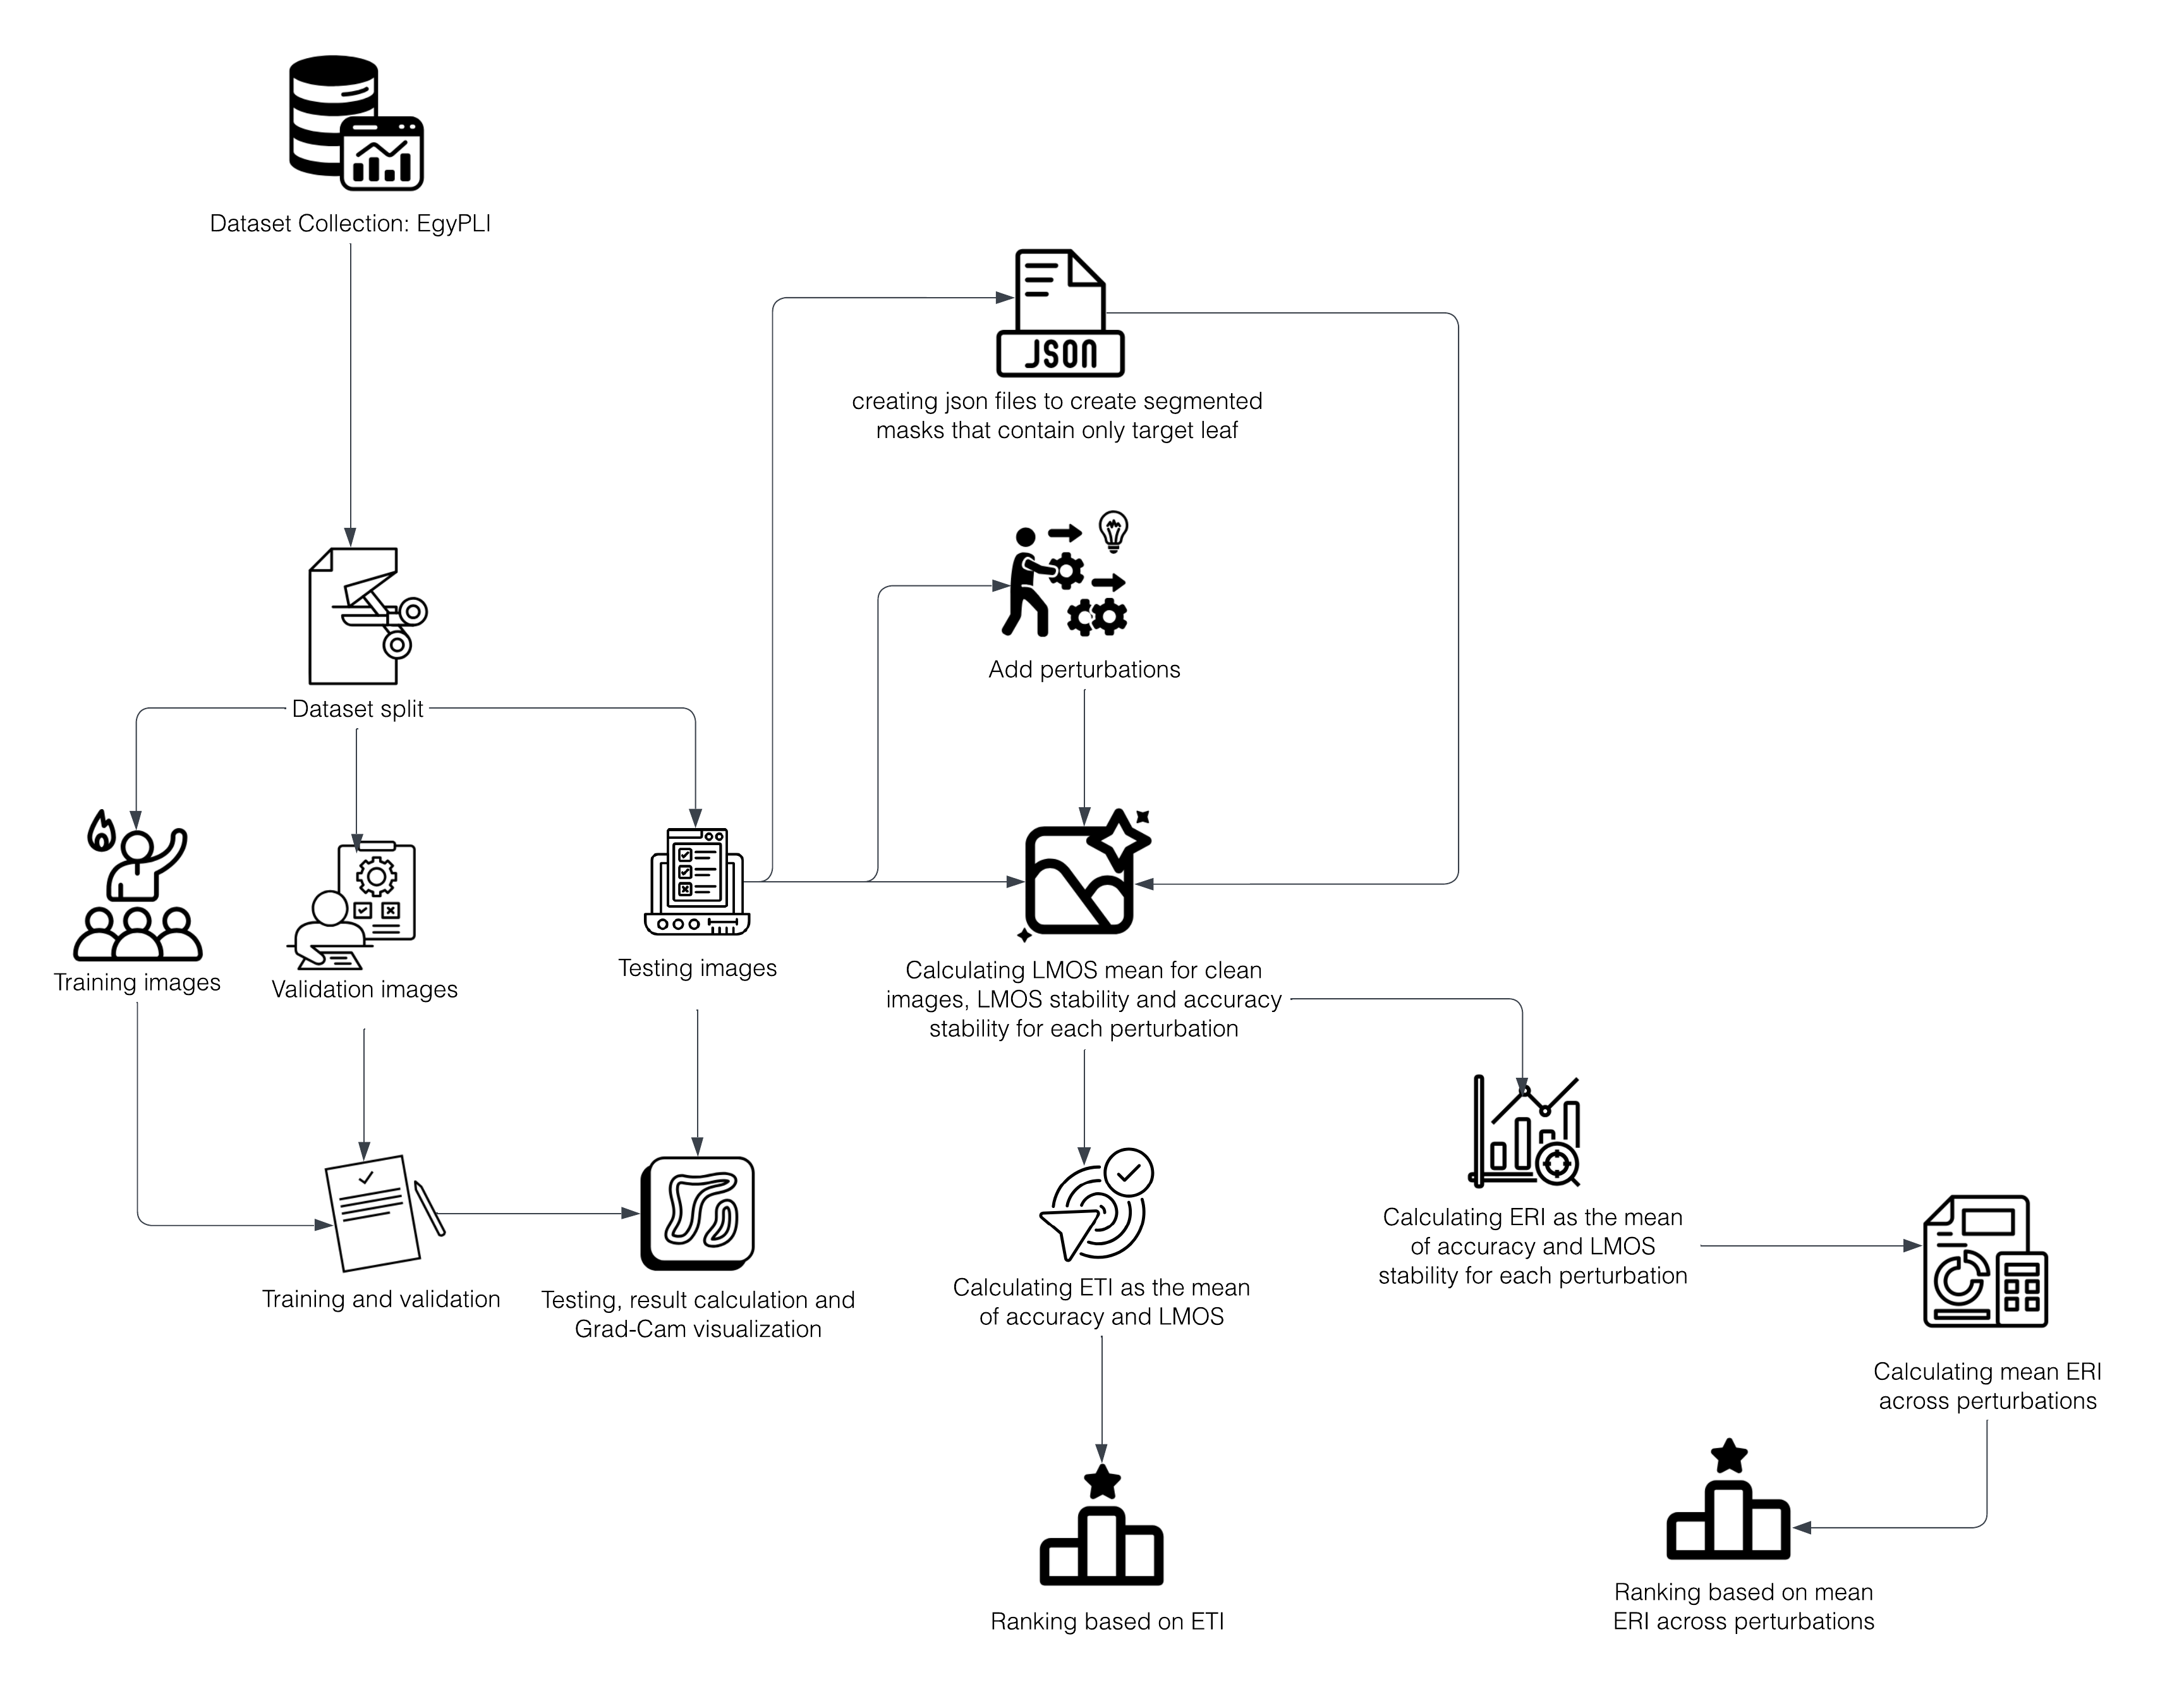
\includegraphics[width=\columnwidth]{Flowchart.png}
    \captionof{figure}{Experimental workflow for trustworthiness and robustness evaluation}
    \label{fig:process_diagram}
\end{center}

The system architecture is described in Figure \ref{fig:process_diagram}. Our framework illustrates the evaluation process of deep learning models. 


The framework begins with the collection of image datasets. The next step is data split. We have split the dataset into training, validation, and testing portions. After that, we have trained CNN models.

The next step is image annotation and adding perturbations. We have annotated the target leaf/flower of each test image and created a corresponding JSON file. From JSON files, segmented masks have been created. We have added various perturbations to the test images. In the following step, we have calculated various scores such as LMOS mean for clean images and LMOS stability mean and accuracy stability under each perturbation. We have also calculated overall mean of accuracy stability and LMOS stability.

Finally, we have calculated ETI for clean images and ERI for each perturbation. Then we have calculated the mean ERI across all perturbations. We have made two rankings of the deep learning models according to ETI and overall ERI.

\section{Experimental Setup}
\subsection{Dataset}
In our research, we have used four publicly available datasets in our empirical study of the proposed evaluation measures: 

\begin{itemize}
\item \textbf{EPLI:} EPLI (officially introduced as EgyPLI in \cite{r10})  contains 3588 images of 8 species (apple, berry, fig, guava, orange, plum, persimmon, and tomato), including both normal and diseased leaves. The images were captured under natural uncontrolled environment. The images are in JPG format and the size is 256*256. The dataset provides image‑level classification labels.

\item \textbf{BDML:} BDML(officially known as BDMediLeaves \cite{r11}) is a dataset of 2,029 original leaf images (augmented to 38,606) from 10 medicinal plant species found in Bangladesh. They were captured with an iPhone 13 under natural light at 3024×4032 resolution. This dataset is designed for machine learning based species identification. We have used the original (not augmented) dataset in this research.

\item \textbf{FLRS:} FLRS (officially Flowers \cite{r12}) is a large image dataset for flower classification. It contains 3,670 training images of five flower species: daisies, tulips, sunflowers, dandelions, and roses. It is available through TensorFlow Datasets (TFDS).

\item \textbf{FRKD:} This dataset (officially Flowers Recognition KAGGLE dataset \cite{r13}) comprises five species: daisy, dandelion, rose, sunflower, and tulip. The raw dataset contains 4317 JPG images (approx. 320×240 pixels) collected from online sources. 
\end{itemize}


\begin{table}[t]
\centering
\caption{Class-wise distribution of the datasets used in this study.}
\label{tab:classwise_dataset_distribution}
\begin{tabular}{|l|r|r|r|r|}
\hline
\multicolumn{5}{|c|}{\textbf{EPLI}} \\
\hline
\textbf{Class} & \textbf{Total} & \textbf{Train} & \textbf{Val} & \textbf{Test} \\
\hline
Apple      & 519 & 415 & 52 & 52 \\
Berry      & 340 & 272 & 34 & 34 \\
Fig        & 508 & 406 & 50 & 52 \\
Guava      & 520 & 416 & 52 & 52 \\
Orange     & 547 & 437 & 55 & 55 \\
Plum       & 468 & 374 & 47 & 47 \\
Persimmon  & 527 & 421 & 53 & 53 \\
Tomato     & 159 & 127 & 16 & 16 \\
\hline
\textbf{Total} & \textbf{3588} & \textbf{2868} & \textbf{359} & \textbf{361} \\
\hline

\multicolumn{5}{|c|}{\textbf{FIRS}} \\
\hline
\textbf{Class} & \textbf{Total} & \textbf{Train} & \textbf{Val} & \textbf{Test} \\
\hline
Daisy       & 633 & 506 & 64 & 63 \\
Dandelion   & 898 & 718 & 90 & 90 \\
Roses       & 641 & 512 & 64 & 65 \\
Sunflowers  & 699 & 560 & 70 & 69 \\
Tulips      & 799 & 639 & 80 & 80 \\
\hline
\textbf{Total} & \textbf{3670} & \textbf{2935} & \textbf{368} & \textbf{367} \\
\hline

\multicolumn{5}{|c|}{\textbf{FRKD}} \\
\hline
\textbf{Class} & \textbf{Total} & \textbf{Train} & \textbf{Val} & \textbf{Test} \\
\hline
Daisy       & 764  & 611 & 76 & 77 \\
Dandelion   & 1052 & 842 & 105 & 105 \\
Roses       & 784  & 627 & 78 & 79 \\
Sunflowers  & 733  & 586 & 73 & 74 \\
Tulips      & 984  & 787 & 98 & 99 \\
\hline
\textbf{Total} & \textbf{4317} & \textbf{3453} & \textbf{430} & \textbf{434} \\
\hline
\end{tabular}
\end{table}

\subsection{Dataset Preparation}
The original (not augmented) BDML dataset is already split into training, validation and testing sets. Other datasets are not split. So we split the other 3 datasets  into training, validation and testing subsets with an approximate ratio of 80\%, 10\% and 10\%. The table \ref{tab:classwise_dataset_distribution} presents the class-wise training, validation, and test splits.

To simplify explainability and localization analysis, the test images have been manually annotated to generate corresponding JSON files. These JSON annotations describe the polygonal boundaries of the target leaf in each image. The JSON files have been converted into binary masks. Here, each mask represents only the target leaf region and excludes the background and other objects in the scene.




\subsection{Training Configuration}

All CNN models have been trained using TensorFlow on a Kaggle environment equipped with two NVIDIA Tesla T4 GPUs. The Custom CNN, VGG16, and ResNet50 architectures and their training settings were adopted from the original EgyPLI study \cite{r10}; while DenseNet121, MobileNetV2, InceptionV3, InceptionResNetV2, and Xception were additionally implemented for the present study following the same transfer learning strategy. The models have been reimplemented using the Keras Functional API instead of the Sequential API used in the original implementation, without modifying the underlying network architectures. For the transfer learning models, ImageNet-pretrained backbones have kept frozen, followed by a global average pooling layer, a dropout layer with a rate of 0.3, and a fully connected layer with 128 ReLU units. The final classification layer has been adjusted according to the number of classes in each dataset. The custom CNN has been implemented from scratch following the architecture adopted in~\cite{r10}. All models have been trained using the Adam optimizer with a learning rate of $5\times10^{-5}$ and categorical cross-entropy loss. An input resolution of $224\times224\times3$ has been used for all models except Xception, which used $299\times299\times3$.





\subsection{Adding Perturbations}

To evaluate the robustness of the proposed framework under distribution shifts and common image corruptions, we have applied nine image perturbations to the test set. As summarized in Table~\ref{tab:perturbations}, these perturbations simulate realistic degradations that may occur during image acquisition, compression, transmission, or environmental variation. The perturbation parameters have been fixed across all experiments to ensure reproducibility and enable fair comparisons among different CNN architectures. The details of the perturbations are shown below:



\noindent\textbf{Gaussian Blur}
Gaussian blur has been applied using a $5 \times 5$ kernel to simulate the loss of fine spatial details caused by defocus or low-quality imaging conditions.

\noindent\textbf{Gaussian Noise}
Additive Gaussian noise with zero mean and standard deviation 0.05 has been introduced to model sensor noise and random intensity fluctuations.

\noindent\textbf{Brightness Adjustment}
Brightness has been increased by adding a constant value of 0.2 to normalized pixel intensities, after which values have been clipped to the valid range $[0,1]$.

% hue shift was 15, made it 10 as in code
\noindent\textbf{Hue Shift}
Hue values in the HSV color space have been shifted by 15 units while preserving the saturation and value channels, simulating color variations caused by illumination or camera characteristics.

% times 1 but here was 0.5
\noindent\textbf{Contrast Adjustment}
Contrast has been modified using mean-centered linear scaling:
\[
I' = (I - \mu_I)\times 0.5 + \mu_I,
\]
where $I$ denotes the input image and $\mu_I$ represents the mean pixel intensity (computed per channel). The resulting values have been clipped to the range $[0,1]$.
% its gamma = 1 in code, here was 2
\noindent\textbf{Gamma Correction}
Nonlinear illumination changes have been simulated using gamma correction:
\[
I' = I^{2.0},
\]
where pixel intensities have been raised to the power of $\gamma = 2.0$.

\noindent\textbf{Motion Blur}
Motion blur has been simulated using a $7 \times 7$ horizontal averaging kernel to emulate camera or object motion during image acquisition.

\noindent\textbf{JPEG Compression}
JPEG compression artifacts have been introduced by encoding and decoding the images with a quality factor of 30, simulating degradation due to lossy storage or transmission.

\noindent\textbf{Random Occlusion}
A randomly positioned rectangular region corresponding to 20\% of the image height and 20\% of the image width has been masked by setting its pixel values to zero, thereby simulating partial object occlusion.


\begin{table}[h]
\centering
\caption{Image perturbation settings used for robustness evaluation.}
\label{tab:perturbations}

\begin{tabular}{|l|l|}
\hline
\textbf{Perturbation Type} & \textbf{Parameter Setting} \\
\hline
Gaussian Blur & $5 \times 5$ kernel \\
Gaussian Noise & Mean = 0, Std = 0.05 \\
Brightness Adjustment & Additive factor = 0.2 \\
Hue Shift & Shift = 15 (HSV) \\
Contrast Adjustment & Factor = 0.5 \\
Gamma Correction & $\gamma = 2.0$ \\
Motion Blur & $7 \times 7$ horizontal kernel \\
JPEG Compression & Quality = 30 \\
Random Occlusion & $20\% \times 20\%$ region masked \\
\hline
\end{tabular}

\end{table}

\subsection {Implementation of the Proposed Measures}

\noindent\textbf{LMOS (Localization
Mask Overlap Score) }

We have proposed the Localization Mask Overlap Score (LMOS) to measure the consistency between model generated explanations and ground-truth object regions. LMOS calculates how much a model focuses on object regions for prediction.

Let $H \in \mathbb{R}^{h \times w}$ denote the Grad-CAM heatmap generated from the last convolutional layer of the network. Its size is h*w. $H$ is resized to the model's input image size.  The resized heatmap size is 299*299 for Xception, 224*224 for others.

A binary attention map is then obtained by thresholding:

\begin{equation}
\hat{H}(i,j) = \mathbb{I}\left( \mathrm{Resize}(H)(i,j) > \tau \right)
\end{equation}
where $\mathbb{I}(\cdot)$ is the indicator function. $\tau$ is the threshold. We set the threshold $0.7$ as we consider only red and yellow pixels to calculate LMOS as those pixels are the most activated and decision-relevant for predictions. $\hat{H}(i,j)$ is a binarized mask representing the activated decision-relevant regions. 

Masks have been created from JSON files of test images and resized into the input image size (299*299 for Xception, 224*224 for others). Let $M \in \{0,1\}^{H \times W}$ denote the resized ground-truth binary segmentation mask. Here, object pixel values are assigned 1, others 0.

The Localization Mask Overlap Score (LMOS) is defined as the proportion of activated decision-relevant regions inside the object region and the  total activated decision-relevant regions. So, LMOS is computed as:
\begin{equation}
\mathrm{LMOS} =
\frac{\sum_{i=1}^{H}\sum_{j=1}^{W} \hat{H}(i,j)\, M(i,j)}
{\sum_{i=1}^{H}\sum_{j=1}^{W} \hat{H}(i,j)}.
\end{equation}

We have derived the mean LMOS, L for all test images.


\noindent\textbf{ETI, Explainable Trustworthy Index}

In order to define trustworthiness, we have proposed  Explainable Trustworthy Index (ETI). ETI of a CNN model combines its accuracy and explainable consistency, mean LMOS. 

Let $acc \in [0,1]$ denote the classification accuracy and $L \in [0,1]$ denote the mean LMOS across all test samples. The ETI is defined as:
\[
\mathrm{ETI} = \frac{acc + L}{2}.
\]



In this study, both components are equally important. Both ${acc}$ and ${L}$ are normalized to the range [0,1] and represent complementary components of model reliability. Accuracy measures predictive performance, whereas ${L}$ measures the mean explanation consistency with the target object. Since neither component alone is sufficient to estimate trustworthiness, equal weighting has been adopted to avoid favoring either predictive performance or explanatory quality.

\noindent\textbf{Ablation Study}

To analyze the ablation study, we have calculated two variants of ETI:

\[
\mathrm{ETI}_{\text{w/o L}} = \frac{acc}{2}, \quad
\mathrm{ETI}_{\text{w/o acc}} = \frac{L}{2}.
\]


\noindent\textbf{Explainable Robustness Index (ERI)}

To evaluate the robustness of classification performance under input perturbations, we measure accuracy stability. Accuracy Stability, denoted by $S_{\text{acc}}$, quantifies the consistency of a model's predictive performance by measuring the similarity between the classification accuracy obtained on perturbed images and that obtained on the corresponding clean test set.

Let $acc_{\text{clean}}$ denote the classification accuracy on the original test set and $acc_{\text{perturbed}}$ denote the classification accuracy obtained on the test set after applying a specific perturbation, p. The accuracy stability under a given perturbation,p is defined as:

\begin{equation}
S_{\text{acc}}^{(p)} = 1 - \frac{|acc_{\text{clean}} - acc_{\text{perturbed}}|}
{acc_{\text{clean}} + acc_{\text{perturbed}} + \epsilon},
\end{equation}

where $\epsilon$ is a small positive constant introduced to avoid division by zero.

A higher value of $S_{\text{acc}}^{(p)}$ indicates that the model maintains its classification performance more consistently under the corresponding perturbed condition. To obtain an overall measure of accuracy stability, the perturbation-specific stability scores are averaged across all $P$ evaluated perturbations as:

\begin{equation}
\overline{S}_{\text{acc}}
=
\frac{1}{P}
\sum_{p=1}^{p}
S_{\text{acc}}^{(p)}
\end{equation}

where $S_{\text{acc}}^{(p)}$ denotes the accuracy stability under the $p$-th perturbation and $P$ is the total number of evaluated perturbations. In this study, $P=9$.

LMOS Stability measures how closely the model's object reliance under perturbation remains to its object reliance on clean images.
To evaluate the robustness under input perturbations, we have measured the stability of LMOS when input images are perturbed.

For each test sample, we have computed LMOS for both the original image and its perturbed version.  Let N be the number of test samples in a test set. Let $LMOS_{\text{clean}}$ denote the LMOS value computed from an original image and $LMOS_{\text{perturbed}}$ denote the LMOS value computed from the corresponding perturbed image.

To quantify the consistency between these two values, we define the LMOS stability under a perturbation:


\begin{equation}
S_{\text{LMOS}} = 1 - \frac{|LMOS_{\text{clean}} - LMOS_{\text{perturbed}}|}{LMOS_{\text{clean}} + LMOS_{\text{perturbed}} + \epsilon},
\end{equation}

where $\epsilon$ is a small constant to avoid division by zero.

A higher value of $S_{\text{LMOS}}$ indicates that the model's reliance on the focus object remains more consistent under the corresponding perturbation. The LMOS stability under a perturbation $p$ is calculated as an average across all $N$ test samples as:

\begin{equation}
{S}_{\text{LMOS}}^{(p)}
=
\frac{1}{N}
\sum_{i=1}^{N}
S_{\text{LMOS},i}^{(p)}
\end{equation}

where $S_{\text{LMOS},i}^{(p)}$ denotes the LMOS stability of the $i$-th test sample under the perturbation $p$, and $N$ represents the total number of test samples.

To obtain an overall mean of LMOS stability across all evaluated perturbations, the perturbation-specific LMOS stability scores are subsequently averaged as:

\begin{equation}
\overline{S}_{\text{LMOS}}
=
\frac{1}{P}
\sum_{p=1}^{P}
{S}_{\text{LMOS}}^{(p)}.
\end{equation}

where $P$ denotes the total number of evaluated perturbations. In this study, $P=9$.



To jointly evaluate the robustness of both classification performance and explainability under input perturbations, we have proposed the \textit{Explainable Robustness Index} (ERI). Unlike accuracy stability and LMOS stability, which separately assess the consistency of predictive performance and model localization behavior, ERI provides a unified measure of robustness by combining the accuracy stability and LMOS stability.

Let ${s}_{\text{acc}}^{{(p)}}$ be accuracy stability and ${s}_{\text{LMOS}}^{{(p)}}$ be LMOS stability under perturbation p. Now, ERI under perturbation p is calculated as:


\begin{equation}
ERI^{{p}} =
\frac{
{S}_{\text{acc}}^{{(p)}}
+
{S}_{\text{LMOS}}^{{(p)}}
}{2}.
\end{equation}

Let $\overline{S}_{\text{acc}}$ denote the overall accuracy stability and $\overline{S}_{\text{LMOS}}$ denote the overall LMOS stability, both obtained by averaging their corresponding perturbation-specific stability scores across the $P$ evaluated perturbations. The proposed ERI is defined as:

\begin{equation}
ERI =
\frac{
\overline{S}_{\text{acc}}
+
\overline{S}_{\text{LMOS}}
}{2}.
\end{equation}

Here, $\overline{S}_{\text{acc}}$ represents the overall consistency of classification accuracy between clean and perturbed inputs, while $\overline{S}_{\text{LMOS}}$ represents the overall consistency of the model's reliance on the focus object under perturbations. Therefore, ERI jointly captures two complementary dimensions of robustness: \textit{predictive stability} and \textit{explanatory stability}.

Since both component scores are bounded in the same range, the resulting ERI also provides a normalized measure of overall robustness. A higher ERI indicates that a model simultaneously maintains its classification performance and preserves its object-focused behavior across the evaluated perturbations. Conversely, a lower ERI indicates that the model exhibits greater instability in one or both dimensions.

\noindent\textbf{Ablation Study}

To analyze the contribution of the individual components of ERI, we calculate two variants by removing one component at a time:

\begin{equation}
\mathrm{ERI}_{\text{w/o LMOS}} =
\frac{\overline{S}_{\text{acc}}}{2},
\qquad
\mathrm{ERI}_{\text{w/o acc}} =
\frac{\overline{S}_{\text{LMOS}}}{2}.
\end{equation}


\begin{table*}[htbp]
\centering
\caption{Representative Grad-CAM visualization strips and LMOS stability analysis across the four benchmark datasets (\texttt{EPLI}, \texttt{BDML},  \texttt{FLRS}, \texttt{FRKD}). Each row displays one composite image strip per model, illustrating inline subpanels for Original, Mask, Segmented target, and Grad-CAM heatmaps under Clean (Pred), Hue, Blur, Contrast, and Compression perturbations with predicted classes and inline LMOS scores.}
\label{tab:gradcam_visualizations}
\setlength{\tabcolsep}{4pt}
\renewcommand{\arraystretch}{1.25}
\resizebox{\textwidth}{!}{%
\begin{tabular}{|c|c|c|c|}
\hline
\textbf{Dataset} & \textbf{Model} & \textbf{Class} & \textbf{Inline Grad-CAM Visualization Strip (Original, Mask, Segmented, Pred, Hue, Blur, Contrast, Compression)} \\
\hline
\multirow{3}{*}{\textbf{EPLI}} 
& Custom CNN & Apple & \raisebox{-0.45\totalheight}{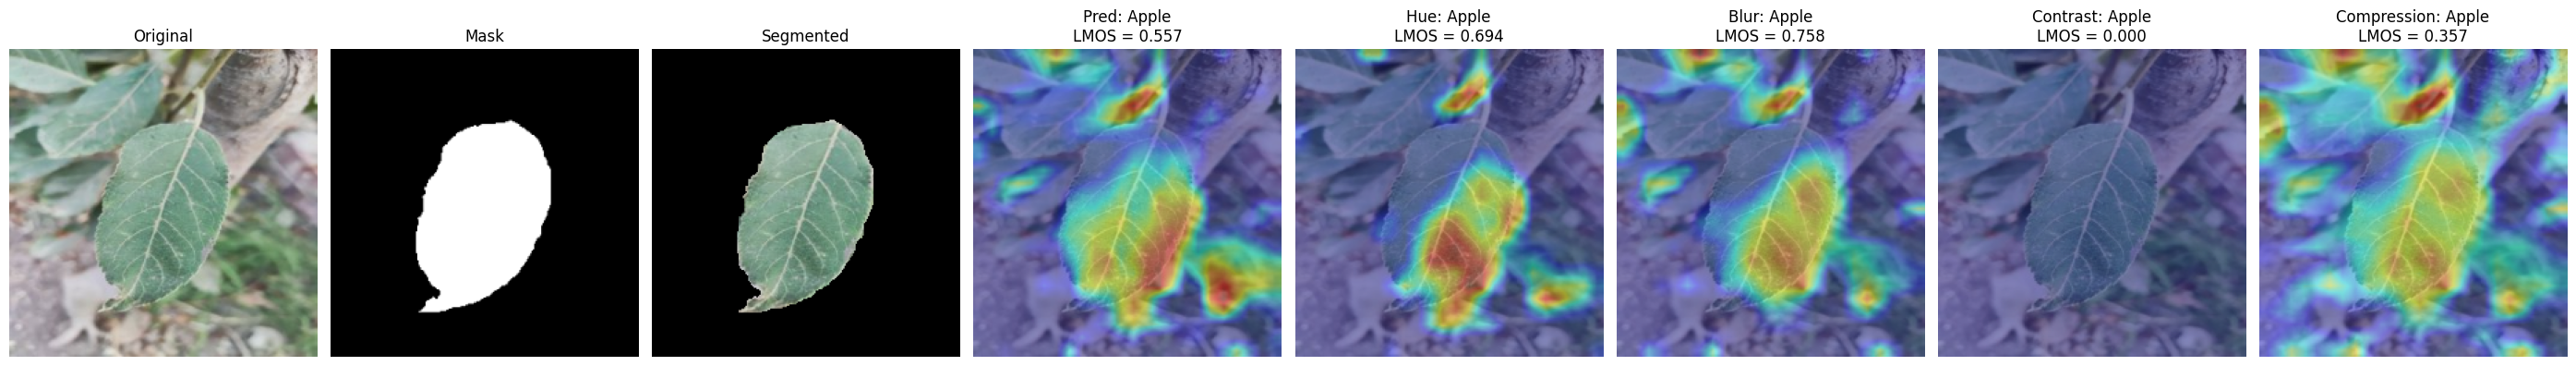
\includegraphics[width=0.72\textwidth]{gradcam-figures/egypli-cnn.png}} \\
\cline{2-4}
& MobilenetV2 & Apple & \raisebox{-0.45\totalheight}{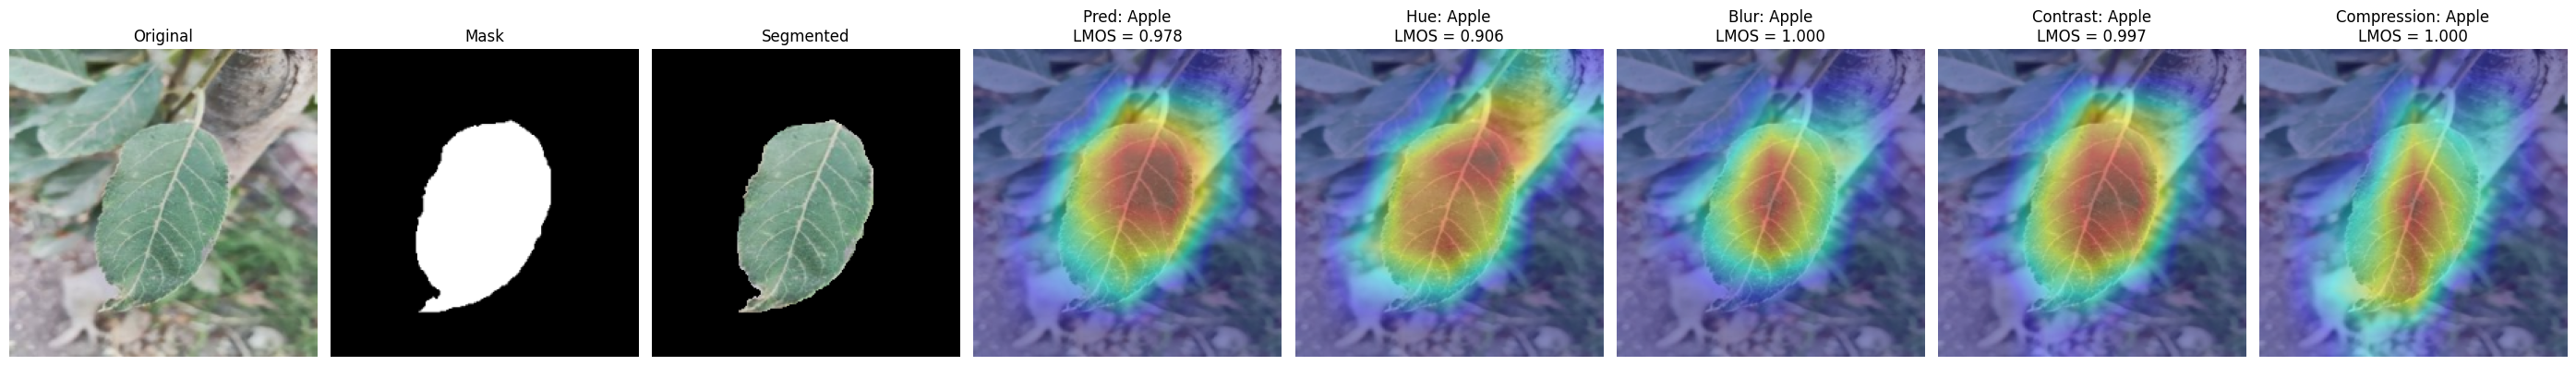
\includegraphics[width=0.72\textwidth]{gradcam-figures/egypli-mobilenetv2.png}} \\
\hline
\multirow{3}{*}{\textbf{BDML}} 
& InceptionV3 & ocimum-tenuiflorum & \raisebox{-0.45\totalheight}{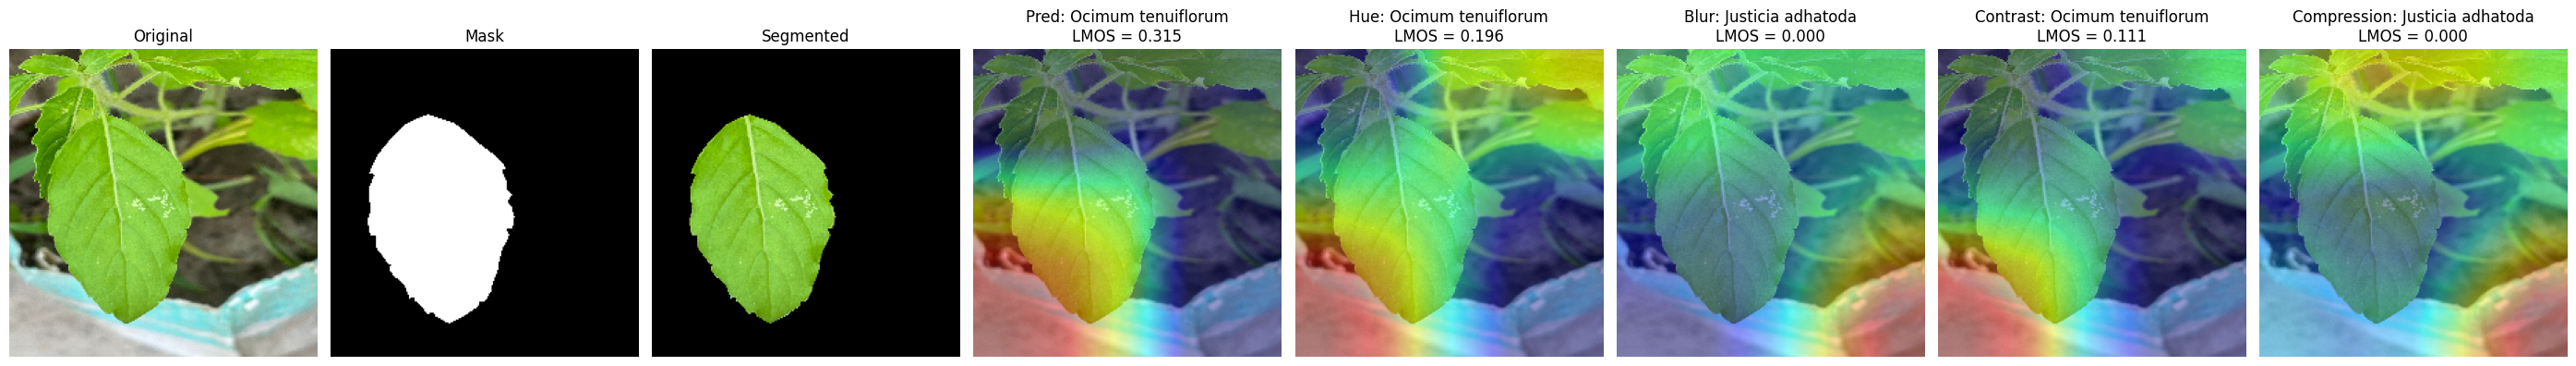
\includegraphics[width=0.72\textwidth]{gradcam-figures/bdmedileaves-inception.png}} \\
\cline{2-4}
& Xception & ocimum-tenuiflorum & \raisebox{-0.45\totalheight}{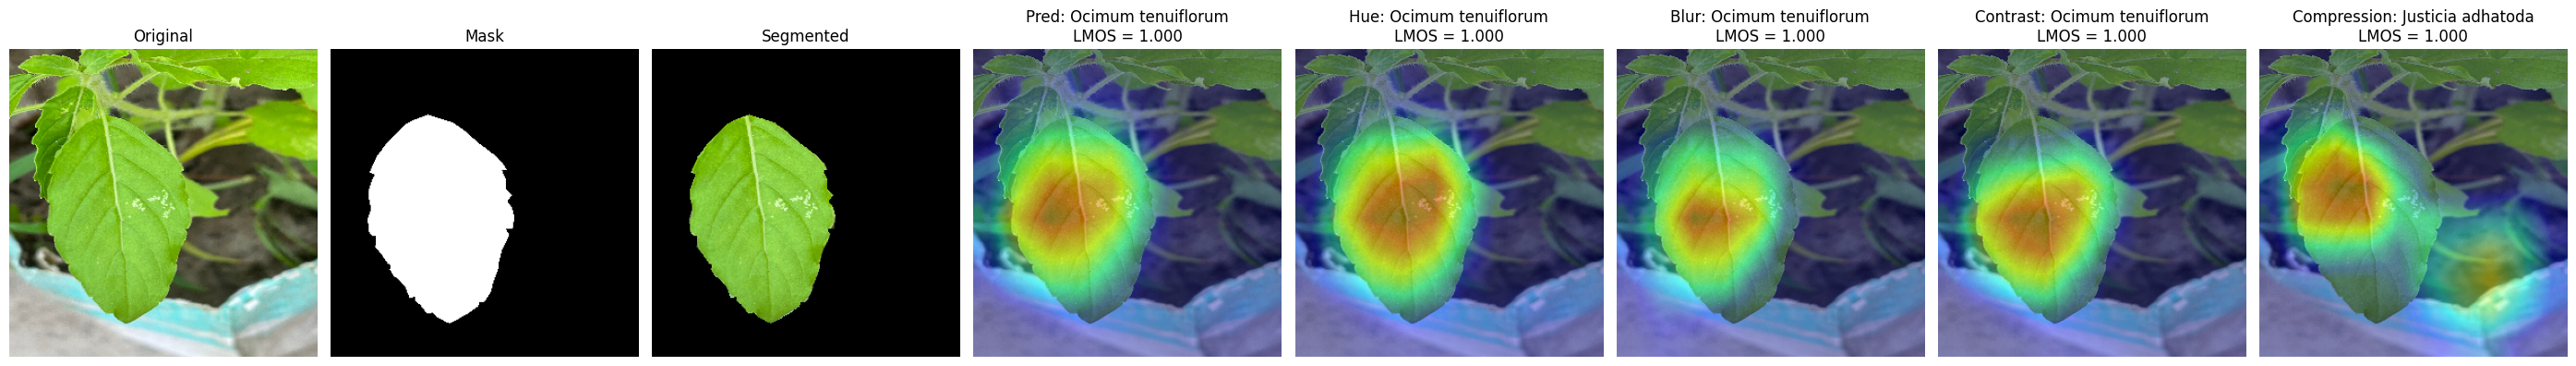
\includegraphics[width=0.72\textwidth]{gradcam-figures/bdmedileaves-xception.png}} \\
\hline
\multirow{3}{*}{\textbf{FLRS}} 
& InceptionV3 & Daisy & \raisebox{-0.45\totalheight}{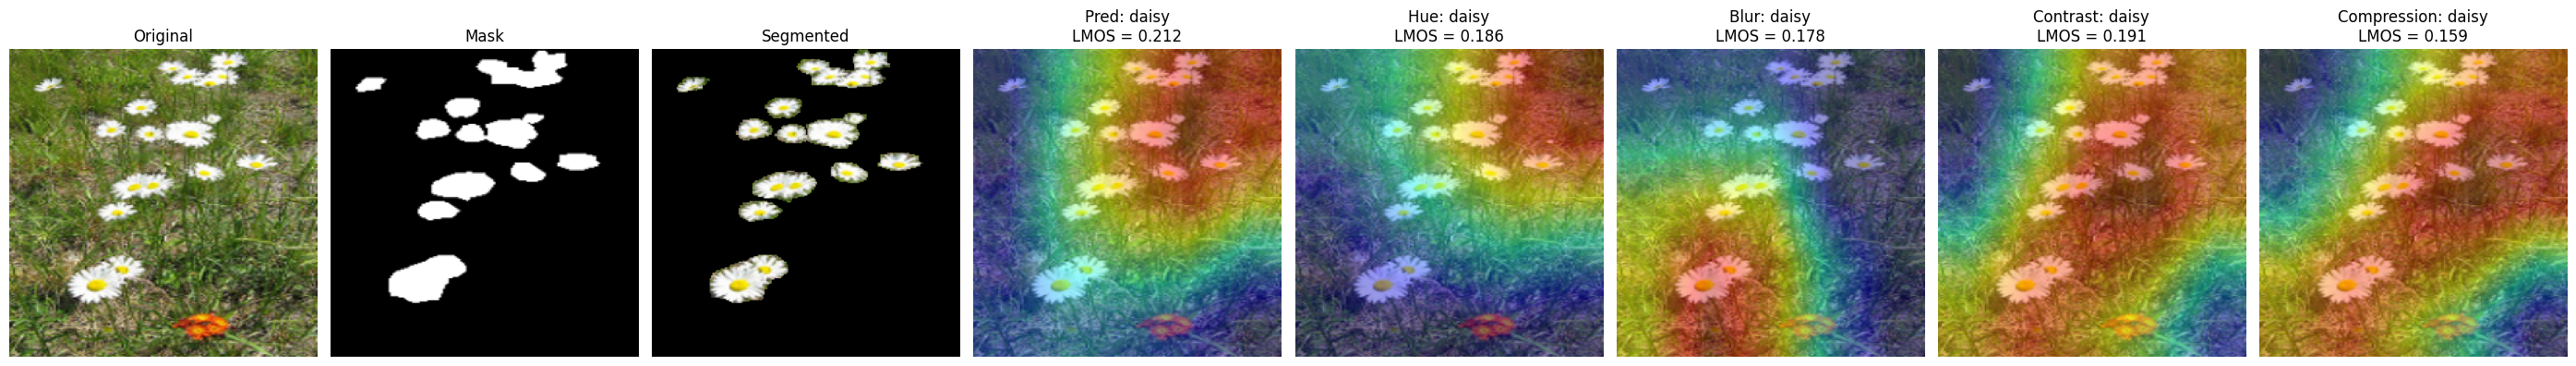
\includegraphics[width=0.72\textwidth]{gradcam-figures/tensorflow-inception.png}} \\
\cline{2-4}
& Xception & Daisy & \raisebox{-0.45\totalheight}{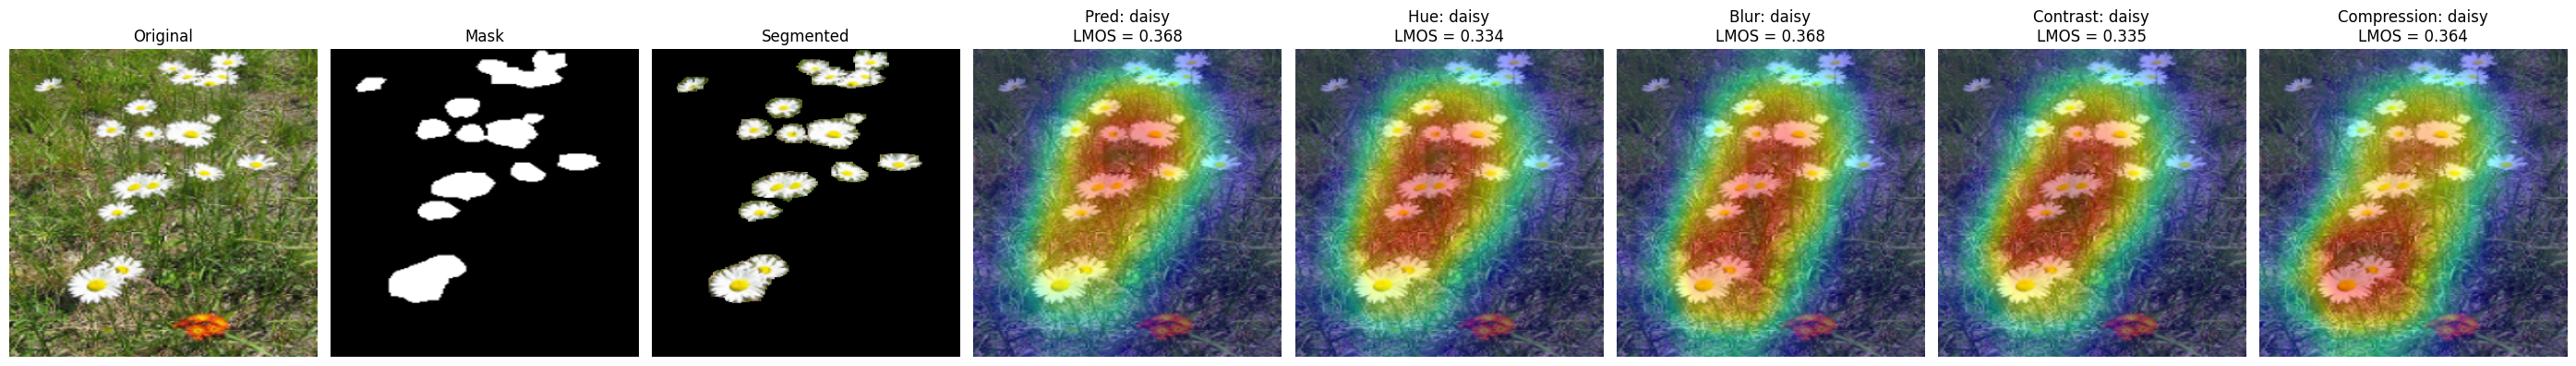
\includegraphics[width=0.72\textwidth]{gradcam-figures/tensorflow-xception.png}} \\
\hline
\multirow{3}{*}{\textbf{FRKD}} 
& Inception V3 & Daisy & \raisebox{-0.45\totalheight}{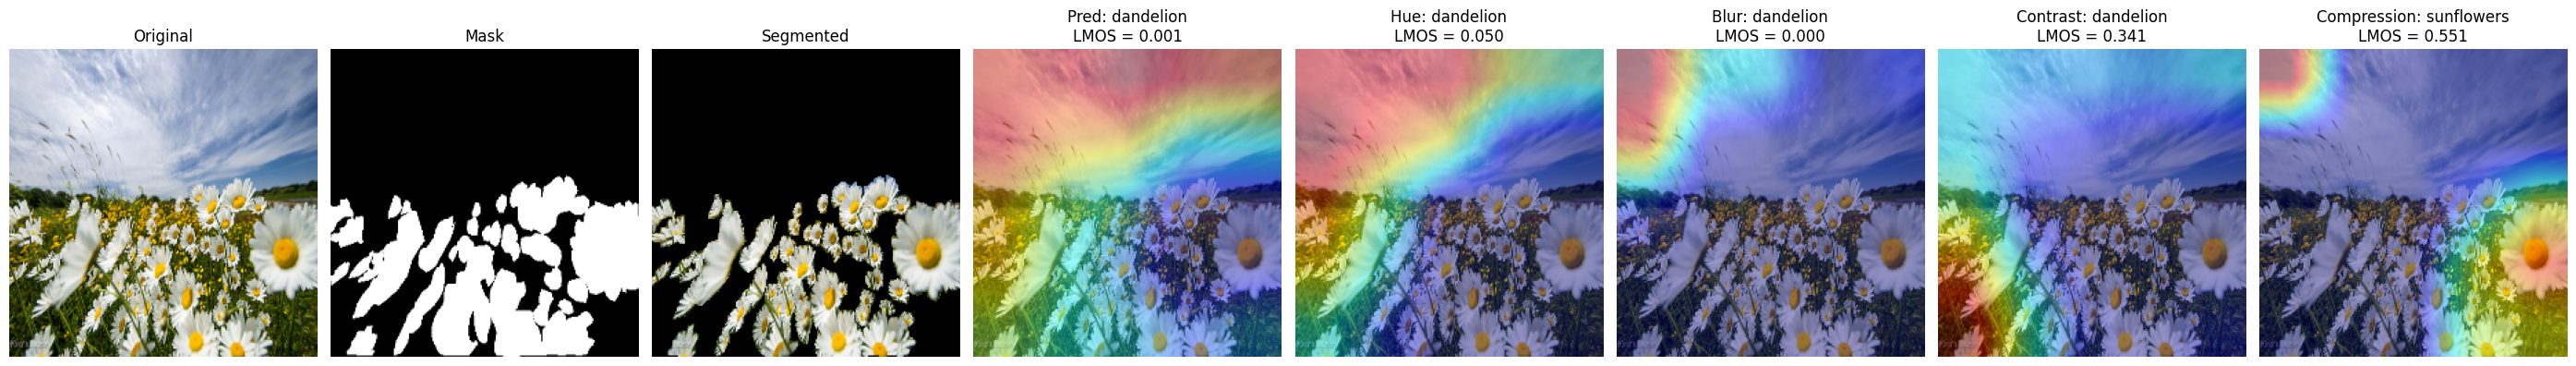
\includegraphics[width=0.72\textwidth]{gradcam-figures/turkish-inception.png}} \\
\cline{2-4}
& Xception & Daisy & \raisebox{-0.45\totalheight}{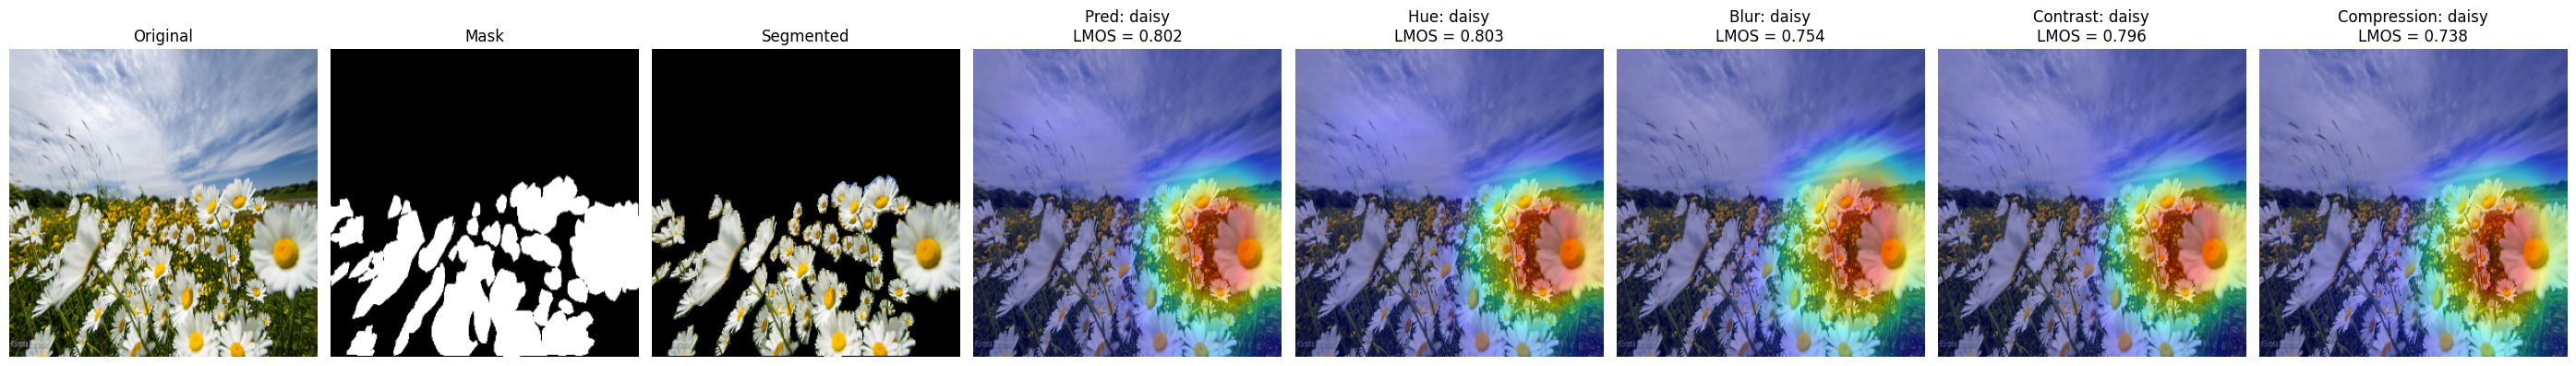
\includegraphics[width=0.72\textwidth]{gradcam-figures/turkish-xception.png}} \\
\hline
\end{tabular}}
\end{table*}




\begin{figure*}[htbp]
\centering
\caption{Visual comparison of Grad-CAM heatmaps under varying binarization thresholds ($\tau \in \{0.5, 0.6, 0.7, 0.8\}$). The optimal threshold $\tau = 0.7$ isolates the core decision-relevant red/yellow regions without introducing peripheral noise ($\tau \le 0.6$) or truncating essential target features ($\tau = 0.8$).}
\label{fig:threshold_comparison}
\vskip 4pt
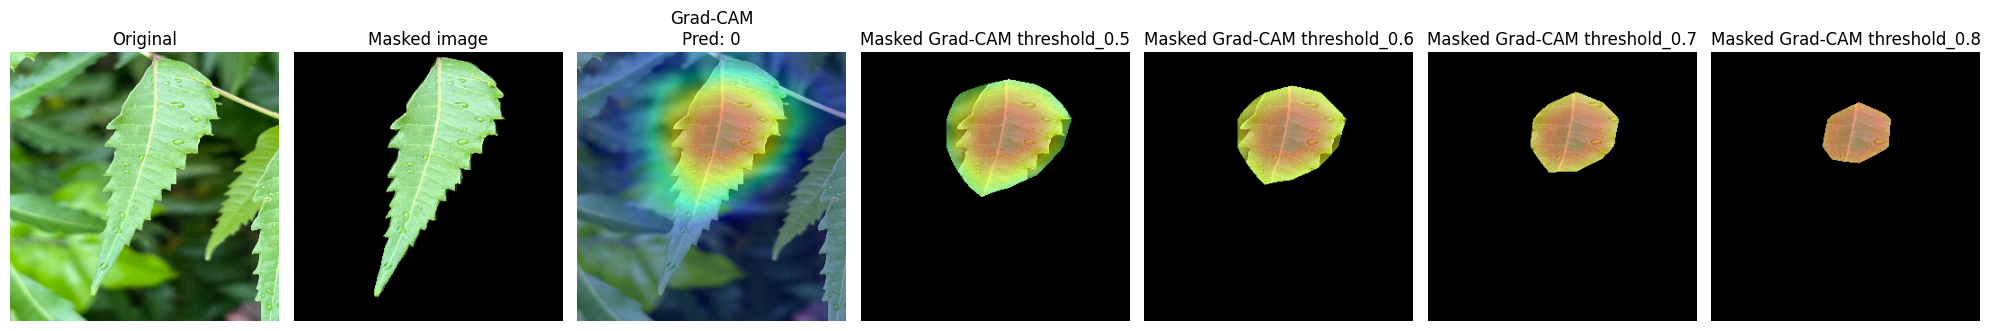
\includegraphics[width=0.98\textwidth]{threshold-figures/image.png}
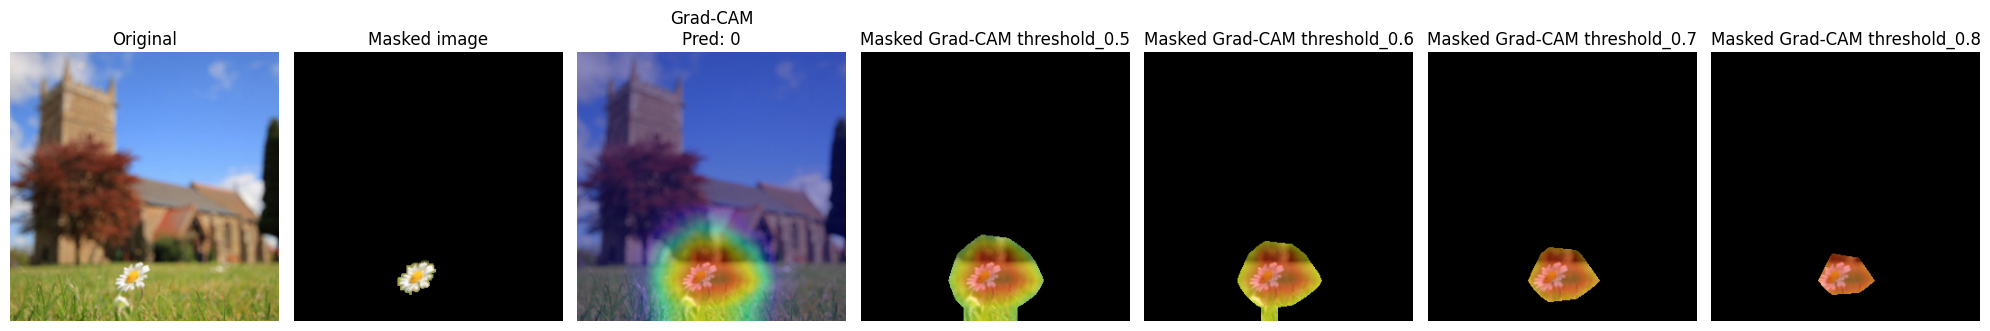
\includegraphics[width=0.98\textwidth]{threshold-figures/12.png}
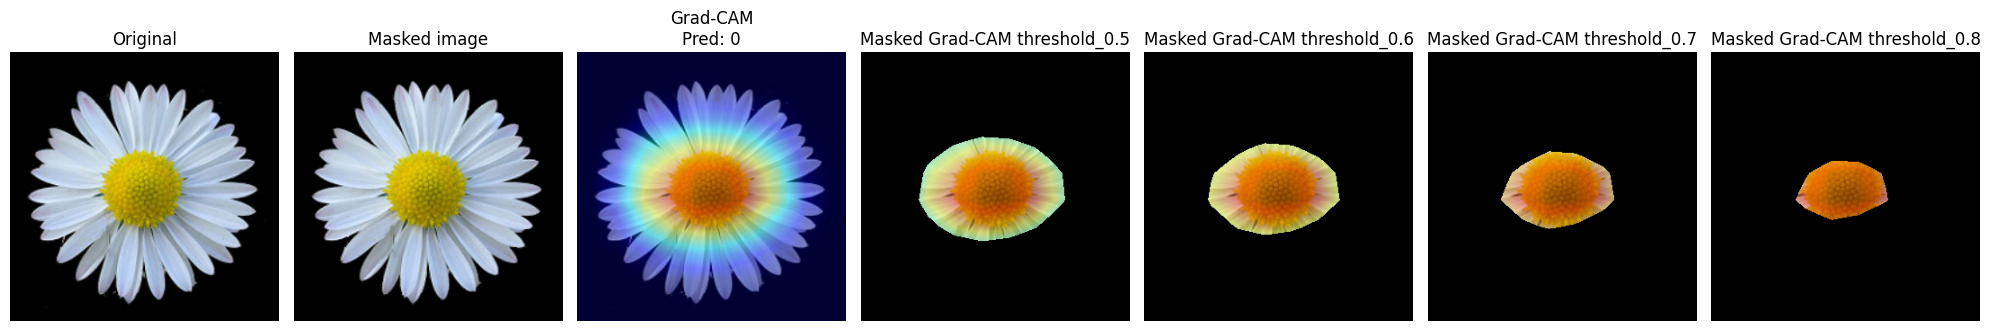
\includegraphics[width=0.98\textwidth]{threshold-figures/16.png}
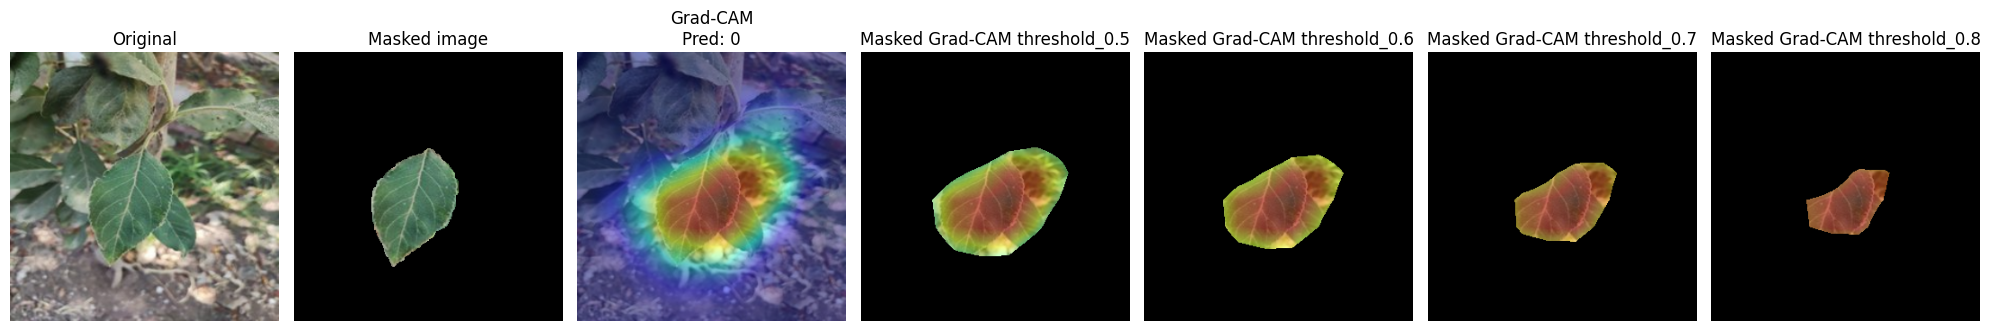
\includegraphics[width=0.98\textwidth]{threshold-figures/4.png}
\end{figure*}



\subsection{Grad-CAM Visualization}
\label{sec:gradcam_visualization}

Table~\ref{tab:gradcam_visualizations} presents representative Grad-CAM visualizations with corresponding LMOS values across the four benchmark datasets. For each selected sample, the visualization strip contains the original input image, its segmentation mask, the segmented target obtained by removing the background, and Grad-CAM visualizations under clean and perturbed conditions. The clean Grad-CAM visualization (Pred) is generated from the original image, whereas the Hue, Blur, Contrast, and Compression panels show the corresponding Grad-CAM responses overlaid on the original image after applying the respective input perturbations. The LMOS value associated with each visualization is also reported inline. This allows the qualitative localization behavior to be quantified. 

The results demonstrate that correct classification does not necessarily imply equivalent localization quality. For example, on the \texttt{EPLI} dataset, both Custom CNN and MobileNetV2 correctly classify an Apple leaf. However, their localization behavior differs significantly. MobileNetV2 has produced a higher LMOS of approximately 0.978, whereas the Custom CNN has obtained an LMOS of approximately 0.557. The Grad-CAM maps of MobileNetV2 overlaid on the original image have exhibited stronger activated regions inside the focus leaf region, while those of Custom CNN have shown a relatively greater portion of activated regions outside or around the focus leaf region. This difference illustrates why classification accuracy alone is insufficient to characterize whether a model provides its prediction based on the appropriate object.

A similar observation is obtained on \texttt{BDML}. Both Inception and Xception correctly predict the representative \textit{Ocimum tenuiflorum} sample, but Xception has achieved a higher LMOS of approximately 1.000 compared with approximately 0.314 for Inception V3. The Xception Grad-CAM maps remain more concentrated on the segmented leaf region, whereas Inception V3 exhibits comparatively more dispersed activation. Thus, models with the same correct prediction can exhibit substantially different degrees of alignment with the target object. The remaining two datasets also represent similar incidents.

The perturbed Grad-CAM visualizations further demonstrate the change of LMOS that encourages calculating localization stability. Under Hue, Blur, Contrast, and Compression perturbations, changes in the activation patterns are accompanied by corresponding changes in LMOS. A model whose LMOS under perturbations is close to that on clean images tends to result in a higher LMOS stability, whereas perturbations that shift LMOS values largely result in lower LMOS stability values. Therefore, the visualization strips provide qualitative evidence for the localization component of the proposed evaluation framework.

Overall, these examples fuel the central motivation of the proposed ETI and ERI metrics: different models produce a correct prediction but may rely on different degrees of decision-relevant region focus. Grad-CAM visualization makes this difference interpretable, while LMOS provides a quantitative measure of the alignment between the model's highlighted regions and the target object. Consequently, the combination of prediction accuracy, localization quality, accuracy and localization stability provides a more informative assessment of CNN reliability than classification accuracy alone.







\subsubsection{Threshold Justification}
\label{sec:threshold_justification}

The selection of the heatmap binarization threshold $\tau$ is important because it determines whether the decision-relevant regions are allowed to pass for heatmap binarization. Figure~\ref{fig:threshold_comparison} presents a visual comparison of some binarized attention maps obtained using $\tau \in {0.5,0.6,0.7,0.8}$. The comparison shows a clear explanation of why the value of $\tau$ should be 0.7.

At $\tau=0.5$, the binarized maps retain a large portion of the heatmap, including not only the highly activated red and yellow regions but also a substantial amount of green regions. Although this threshold preserves more activated pixels, the inclusion of weakly activated peripheral regions may introduce non-decision-relevant areas into the masked Grad-CAM. Consequently, it may raise a question whether heatmap binarization masks only allow decision-relevant regions.

Increasing the threshold to $\tau=0.6$ significantly reduces the inclusion of green regions. However, some green activations remain in the binarized attention maps. This indicates that the resulting mask still allows relatively weakly activated regions to pass in addition to the strongly activated areas. Thus, $\tau=0.6$ provides improved selectivity compared with $\tau=0.5$, but is not sufficient to isolate the most strongly activated regions.

At $\tau=0.7$, the binarization primarily allows only the red and yellow regions of the Grad-CAM heatmap. These regions correspond to the highly activated maps and therefore represent the most decision-relevant areas for the model's prediction. At the same time, the threshold avoids retaining weaker green activations. As illustrated in Figure~\ref{fig:threshold_comparison}, $\tau=0.7$ therefore provides a suitable balance between excluding peripheral low-intensity activation and preserving the core regions highlighted by Grad-CAM.

In contrast, $\tau=0.8$ produces a substantially more restrictive attention mask. At this threshold, predominantly red regions and only limited portions of yellow regions are retained. Although this increases the selectivity of the attention map, it can also remove some highly activated regions that are included in decision-relevant regions. Therefore, $\tau=0.8$ may excessively restrict the decision-relevant region.

Based on this qualitative comparison, $\tau=0.7$ has been selected for LMOS computation. This threshold retains the core red/yellow activated regions, excluding most of the lower-intensity green regions, providing a practical balance between sensitivity and relevant target features. The same threshold is applied consistently across all datasets, models, and test images to ensure that LMOS values remain comparable.



\section{Result and Discussion}

\subsection{Explainable Trustworthiness Index (ETI)}

Table~\ref{tab:eti_all_datasets} illustrates a detailed evaluation of the proposed Explainable Trustworthiness Index (ETI) across four benchmark datasets: EPLI, BDML, FLRS, and FRKD. ETI not only considers accuracy but also explanation quality. It integrates prediction accuracy and the mean Localization Mask Overlap Score (LMOS). Therefore, a model achieves a higher ETI only when it possesses both reliable classification capability and consistent focus on semantically meaningful image regions instead of background. The results clearly indicate that accuracy alone is not enough to measure model trustworthiness. Several models have achieved competitive classification performance but fail to achieve higher ETI values due to poor localization quality.


\begin{table*}[htbp]
\centering
\caption{Comparison of classification accuracy, mean LMOS, ETI, and ablation variants across different CNN architectures on four benchmark datasets.}
\label{tab:eti_all_datasets}
\resizebox{\textwidth}{!}{%
\footnotesize
\begin{tabular}{|l|c|l|c|c|c|c|c|}
\hline
\textbf{Dataset} & \textbf{Rank} & \textbf{Model} & 
\textbf{Accuracy} & \textbf{LMOS} & 
\textbf{ETI} & \textbf{ETI w/o Acc.} & 
\textbf{ETI w/o LMOS} \\
\hline

\multirow{8}{*}{EPLI}
&1&MobileNetV2&0.9945&0.7765&0.8855&0.3882&0.4972\\
&2&Xception&0.9945&0.7638&0.8791&0.3819&0.4972\\
&3&DenseNet121&1.0000&0.6964&0.8482&0.3482&0.5000\\
&4&InceptionResNetV2&0.9889&0.5529&0.7709&0.2764&0.4945\\
&5&VGG16&0.9834&0.5268&0.7551&0.2634&0.4917\\
&6&InceptionV3&0.9917&0.3617&0.6767&0.1809&0.4958\\
&7&ResNet50&0.6122&0.7256&0.6689&0.3628&0.3061\\
&8&Custom CNN&0.9945&0.1900&0.5922&0.0950&0.4972\\
\hline

\multirow{8}{*}{BDML}
&1&MobileNetV2&0.9703&0.7611&0.8657&0.3805&0.4851\\
&2&Xception&0.9505&0.7800&0.8653&0.3900&0.4752\\
&3&DenseNet121&0.9802&0.7118&0.8460&0.3559&0.4901\\
&4&VGG16&0.8960&0.5873&0.7416&0.2936&0.4480\\
&5&InceptionResNetV2&0.9059&0.5184&0.7122&0.2592&0.4530\\
&6&InceptionV3&0.9307&0.3344&0.6325&0.1672&0.4653\\
&7&ResNet50&0.4604&0.7817&0.6211&0.3909&0.2302\\
&8&Custom CNN&0.7376&0.3310&0.5343&0.1655&0.3688\\
\hline

\multirow{8}{*}{ FLRS}
&1&Xception&0.8828&0.6869&0.7849&0.3435&0.4414\\
&2&DenseNet121&0.9046&0.6188&0.7617&0.3094&0.4523\\
&3&MobileNetV2&0.8665&0.5958&0.7311&0.2979&0.4332\\
&4&VGG16&0.8147&0.6311&0.7229&0.3155&0.4074\\
&5&InceptionResNetV2&0.8501&0.5581&0.7041&0.2791&0.4251\\
&6&InceptionV3&0.8229&0.3749&0.5989&0.1875&0.4114\\
&7&ResNet50&0.5123&0.5623&0.5373&0.2812&0.2561\\
&8&Custom CNN&0.7003&0.2891&0.4947&0.1446&0.3501\\
\hline

\multirow{8}{*}{FRKD}
&1&Xception&0.9032&0.6029&0.7531&0.3015&0.4516\\
&2&DenseNet121&0.9124&0.5382&0.7253&0.2691&0.4562\\
&3&VGG16&0.8387&0.5786&0.7087&0.2893&0.4194\\
&4&MobileNetV2&0.8986&0.5091&0.7038&0.2545&0.4493\\
&5&InceptionResNetV2&0.8894&0.4705&0.6800&0.2353&0.4447\\
&6&InceptionV3&0.8825&0.3063&0.5944&0.1531&0.4412\\
&7&ResNet50&0.4977&0.4769&0.4873&0.2384&0.2488\\
&8&Custom CNN&0.6820&0.2714&0.4767&0.1357&0.3410\\

\hline
\end{tabular}}
\end{table*}



For the EPLI dataset, MobileNetV2 and Xception have achieved the highest ETI values of 0.8855 and 0.8791, respectively, despite DenseNet121 obtaining the highest classification accuracy of 1.0000. Although DenseNet121 perfectly classifies all test samples, its lower LMOS value (0.6964) reduces its overall ETI to 0.8482. This observation highlights the importance of explanation consistency as well as predictive accuracy for trustworthiness. Similarly, the Custom CNN achieves a high accuracy of 0.9945, which is comparable to the best-performing architectures. However, its LMOS value is the lowest (0.1900). So ultimately the ETI value is the lowest (0.5922). This indicates that the model may rely on irrelevant image regions rather than the focus leaf regions for decision-making.

A similar trend is observed on the BDML dataset. MobileNetV2 and Xception provide the highest ETI scores of 0.8657 and 0.8653, respectively, showing balanced classification capability and explanation reliability. In contrast, DenseNet121 achieves the highest accuracy among the evaluated models (0.9802), but its lower LMOS value (0.7118) limits its ETI performance (0.8460). The results further demonstrate that models with slightly lower accuracy can outperform highly accurate models when they generate more meaningful visual explanations. For example, Xception achieves lower accuracy than DenseNet121 but obtains nearly highest ETI due to superior localization behavior.

For the flower classification datasets, the ETI analysis reveals similar but dataset-dependent behavior. On the FLRS dataset, Xception achieves the highest ETI score of 0.7849, followed by DenseNet121 (0.7617) and MobileNetV2 (0.7311). Although DenseNet121 provides the highest accuracy (0.9046), Xception achieves better overall trustworthiness due to its higher LMOS value (0.6869). The FRKD also demonstrates the effectiveness of ETI in distinguishing models with similar predictive performance. Xception achieves the highest ETI score (0.7531), while DenseNet121 obtains the highest accuracy (0.9124). However, the lower LMOS of DenseNet121 (0.5382) reduces its ETI to 0.7253. These results confirm that the proposed metric provides additional insights beyond conventional accuracy ranking.

The ablation results shown in Figure \ref{tab:eti_all_datasets} further validate the contribution of both components of ETI. The ``ETI without accuracy'' variant, which considers only LMOS information, produces substantially lower values across all datasets because explanation quality alone cannot represent complete model reliability. Similarly, the ``ETI without LMOS'' variant, which depends only on classification accuracy, fails to capture whether the model focuses on meaningful regions. For instance, in the EPLI dataset, the Custom CNN achieves an accuracy-based ETI value of 0.4972 when LMOS is removed, which incorrectly suggests competitive trustworthiness compared with stronger architectures. However, the complete ETI value decreases to 0.5922 due to its poor localization capability. This demonstrates that LMOS provides essential complementary information that cannot be obtained from accuracy alone.

Across all datasets, the ablation trends consistently show that the complete ETI formulation produces a more balanced and discriminative evaluation compared with either individual component. The integration of accuracy and LMOS prevents the possibility of overestimation of models that achieve high classification scores through potentially unreliable visual reasoning. Overall, the experimental results from Table~\ref{tab:eti_all_datasets} demonstrate that ETI provides a more comprehensive measurement of CNNs by simultaneously evaluating predictive reliability and explanation quality.


\begin{table*}[t]
\centering
\caption{Accuracy stability of different CNN architectures on EPLI under various input perturbations.}
\label{tab:accuracy_stability_egypli}

\scriptsize
\setlength{\tabcolsep}{3pt}
\renewcommand{\arraystretch}{1.1}

\begin{tabular}{|l|ccccccccc|c|}
\hline
\textbf{Model} &
\textbf{Noise} &
\textbf{Blur} &
\textbf{Brightness} &
\textbf{Hue} &
\textbf{Contrast} &
\textbf{Gamma} &
\textbf{Motion Blur} &
\textbf{Compression} &
\textbf{Occlusion} &
\textbf{Mean}\\
\hline

Custom CNN
&0.9801&0.9958&0.9021&0.8711&0.8494&0.8033&0.9916&0.9986&0.9801&0.9302\\

DenseNet121
&0.9944&0.9845&1.0000&0.9986&0.9860&0.9916&0.9159&0.9930&1.0000&0.9849\\

MobileNetV2
&0.9441&0.9534&1.0000&0.9916&0.9902&0.9986&0.8816&0.9916&0.9830&0.9704\\

InceptionResNetV2
&0.9727&0.9829&0.9986&0.9986&0.9944&0.9915&0.9149&0.9887&0.9469&0.9766\\

InceptionV3
&0.9593&0.9771&0.9958&0.9972&0.9944&0.9915&0.9217&0.9757&0.9201&0.9703\\

ResNet50
&0.9816&0.6962&0.9955&0.9862&0.4599&0.8978&0.5316&0.9769&0.9113&0.8263\\

VGG16
&0.9828&0.9695&0.9958&0.9813&0.8380&0.9843&0.8284&0.9943&0.9481&0.9469\\

Xception
&0.9801&0.9902&0.9986&1.0000&0.9972&0.9958&0.9549&0.9958&0.9859&0.9887\\

\hline
\end{tabular}
\end{table*}


\begin{table*}[t]
\centering
\caption{LMOS stability of different CNN architectures on EPLI under various input perturbations.}
\label{tab:lmos_stability_egypli}

\scriptsize
\setlength{\tabcolsep}{3pt}
\renewcommand{\arraystretch}{1.1}

\begin{tabular}{|l|ccccccccc|c|}
\hline
\textbf{Model} &
\textbf{Noise} &
\textbf{Blur} &
\textbf{Brightness} &
\textbf{Hue} &
\textbf{Contrast} &
\textbf{Gamma} &
\textbf{Motion Blur} &
\textbf{Compression} &
\textbf{Occlusion} &
\textbf{Mean}\\
\hline

Custom CNN
&0.7525&0.7421&0.5343&0.5701&0.4545&0.5053&0.7242&0.9071&0.7376&0.6586\\

DenseNet121
&0.8322&0.8151&0.9352&0.8723&0.8256&0.8398&0.6551&0.8103&0.8402&0.8251\\

MobileNetV2
&0.8099&0.8200&0.9303&0.8910&0.8382&0.8763&0.7212&0.8393&0.8373&0.8404\\

InceptionResNetV2
&0.6846&0.6978&0.8646&0.8556&0.7867&0.7693&0.5969&0.7433&0.7177&0.7463\\

InceptionV3
&0.6550&0.6384&0.8425&0.8184&0.7378&0.7450&0.5560&0.6294&0.6426&0.6961\\

ResNet50
&0.8417&0.7607&0.9332&0.9070&0.7830&0.8010&0.7666&0.8410&0.8187&0.8281\\

VGG16
&0.7576&0.7014&0.8812&0.7836&0.5362&0.7432&0.5007&0.7693&0.6564&0.7033\\

Xception
&0.8540&0.8611&0.9482&0.9489&0.9122&0.8802&0.7613&0.8712&0.8877&0.8805\\


\hline
\end{tabular}
\end{table*}

\begin{table*}[t]
\centering
\caption{ERI of different CNN architectures on EPLI under individual input perturbations.}
\label{tab:eri_perturbation_egypli}

\scriptsize
\setlength{\tabcolsep}{4pt}
\renewcommand{\arraystretch}{1.1}

\begin{tabular}{|l|ccccccccc|c|}
\hline
\textbf{Model} &
\textbf{Noise} &
\textbf{Blur} &
\textbf{Brightness} &
\textbf{Hue} &
\textbf{Contrast} &
\textbf{Gamma} &
\textbf{Motion Blur} &
\textbf{Compression} &
\textbf{Occlusion} &
\textbf{Overall ERI}\\
\hline

Custom CNN
&0.8663&0.8690&0.7182&0.7206&0.6520&0.6543&0.8579&0.9528&0.8589&0.7944\\

DenseNet121
&0.9133&0.8998&0.9676&0.9355&0.9058&0.9157&0.7855&0.9017&0.9201&0.9050\\

MobileNetV2
&0.8770&0.8867&0.9651&0.9413&0.9142&0.9375&0.8014&0.9155&0.9102&0.9054\\

InceptionResNetV2
&0.8286&0.8403&0.9316&0.9271&0.8905&0.8804&0.7559&0.8660&0.8323&0.8614\\

InceptionV3
&0.8072&0.8077&0.9192&0.9078&0.8661&0.8682&0.7389&0.8025&0.7813&0.8332\\

ResNet50
&0.9117&0.7285&0.9644&0.9466&0.6215&0.8494&0.6491&0.9089&0.8650&0.8272\\

VGG16
&0.8702&0.8355&0.9385&0.8824&0.6871&0.8638&0.6645&0.8818&0.8023&0.8251\\

Xception
&0.9170&0.9256&0.9734&0.9745&0.9547&0.9380&0.8581&0.9335&0.9368&0.9346\\

\hline
\end{tabular}
\end{table*}


\begin{table*}[t]
\centering
\caption{ERI ranking and ablation analysis of CNN architectures on EPLI}
\label{tab:eri_ablation_ranking_egypli}

\scriptsize
\setlength{\tabcolsep}{5pt}
\renewcommand{\arraystretch}{1.15}

\begin{tabular}{|c|l|c|c|c|c|c|}
\hline
\textbf{Rank} &
\textbf{Model} &
\textbf{Accuracy Stability (mean)} &
\textbf{LMOS Stability (mean)} &
\textbf{ERI} &
\textbf{ERI w/o Accuracy} &
\textbf{ERI w/o LMOS} \\
\hline

1 & Xception
&0.9887&0.8805&0.9346&0.4403&0.4944\\

2 & MobileNetV2
&0.9704&0.8404&0.9054&0.4202&0.4852\\

3 & DenseNet121
&0.9849&0.8251&0.9050&0.4125&0.4924\\

4 & InceptionResNetV2
&0.9766&0.7463&0.8614&0.3731&0.4883\\

5 & InceptionV3
&0.9703&0.6961&0.8332&0.3481&0.4852\\

6 & ResNet50
&0.8263&0.8281&0.8272&0.4140&0.4132\\

7 & VGG16
&0.9469&0.7033&0.8251&0.3517&0.4735\\

8 & Custom CNN
&0.9302&0.6586&0.7944&0.3293&0.4651\\

\hline
\end{tabular}
\end{table*}


\subsection{Explainable Robustness Index (ERI)}

\noindent\textbf{EPLI}

The ERI values of the evaluated CNN architectures have been assessed from both prediction stability and explanation stability. Table~\ref{tab:accuracy_stability_egypli} shows that most architectures have maintained high accuracy stability under common perturbations, particularly brightness, hue, gamma, and compression. Xception has achieved the highest mean accuracy stability (0.9887), followed by DenseNet121 (0.9849) and InceptionResNetV2 (0.9766). In contrast, ResNet50 has exhibited substantially lower stability (0.8263), mainly due to its sensitivity to blur, contrast, and motion blur. Although the Custom CNN has maintained a relatively high mean accuracy stability of 0.9302, its performance does not necessarily indicate reliable robustness when the stability of its explanations is considered.

Table~\ref{tab:lmos_stability_egypli} reveals greater variation in explanation stability across architectures. Xception has achieved the highest mean LMOS stability (0.8805), followed by MobileNetV2 (0.8404) and ResNet50 (0.8281). The Custom CNN has shown considerably lower LMOS stability (0.6586), indicating that its Grad-CAM explanations have changed more substantially under perturbations despite relatively stable predictions. Motion blur generally has produced the largest degradation in explanation stability, while brightness and hue shifts are comparatively less disruptive for most architectures.

The combined results are reflected in the ERI values in Table~\ref{tab:eri_perturbation_egypli}. Xception has achieved the highest overall ERI of 0.9346, demonstrating a strong balance between prediction and explanation stability across all perturbations. MobileNetV2 (0.9054) and DenseNet121 (0.9050) have followed closely. At the other end of the ranking, the Custom CNN has obtained the lowest ERI (0.7944), despite achieving a substantially higher accuracy stability than ResNet50. This demonstrates the importance of incorporating explanation stability into robustness assessment: high predictive stability alone does not guarantee stable and trustworthy model behavior. Across perturbations, brightness and hue generally have produced the highest ERI values, whereas motion blur is consistently among the most challenging perturbations.

The ranking and ablation results in Table~\ref{tab:eri_ablation_ranking_egypli} further support this observation. Xception has ranked first with an ERI of 0.9346, while MobileNetV2 and DenseNet121 have ranked second and third, respectively. Removing either accuracy stability or LMOS stability substantially reduces the resulting score for every architecture, confirming that both components contribute meaningfully to the proposed ERI. Overall, the EPLI results demonstrate that ERI provides a more comprehensive characterization of CNN robustness by jointly considering whether predictions remain stable and whether the corresponding visual explanations remain consistent under input perturbations.
\\
\\
\\


\begin{table*}[t]
\centering
\caption{Accuracy stability of different CNN architectures on BDML under various input perturbations.}
\label{tab:accuracy_stability_bdmedileaves}

\scriptsize
\setlength{\tabcolsep}{3pt}
\renewcommand{\arraystretch}{1.1}

\begin{tabular}{|l|ccccccccc|c|}
\hline
\textbf{Model} &
\textbf{Noise} &
\textbf{Blur} &
\textbf{Brightness} &
\textbf{Hue} &
\textbf{Contrast} &
\textbf{Gamma} &
\textbf{Motion Blur} &
\textbf{Compression} &
\textbf{Occlusion} &
\textbf{Mean} \\
\hline

Custom CNN
&0.9689&0.7265&0.7319&0.8359&0.5174&0.8221&0.5943&0.9724&0.9084&0.7864\\

DenseNet121
&0.9794&0.9496&0.9924&0.9846&0.9846&0.9898&0.8750&0.9714&0.9714&0.9665\\

MobileNetV2
&0.9792&0.9111&0.9949&1.0000&0.9871&0.9949&0.8085&0.9574&0.9377&0.9523\\

InceptionResNetV2
&0.9513&0.9360&0.9917&0.9917&0.9890&0.9973&0.8738&0.9204&0.9452&0.9552\\

InceptionV3
&0.9810&0.9379&0.9838&0.9920&0.9865&0.9973&0.8876&0.9195&0.9038&0.9544\\

ResNet50
&0.9780&0.4103&0.8929&0.9738&0.3966&0.8929&0.4103&0.9186&0.9249&0.7553\\

VGG16
&1.0000&0.9538&0.9916&0.9803&0.8997&0.9745&0.8131&0.9888&0.9716&0.9526\\

Xception
&0.9760&0.8739&0.9895&0.9921&0.9868&0.9948&0.8805&0.9122&0.9183&0.9471\\

\hline
\end{tabular}
\end{table*}

\begin{table*}[t]
\centering
\caption{LMOS stability of different CNN architectures on BDML under various input perturbations.}
\label{tab:lmos_stability_bdmedileaves}

\scriptsize
\setlength{\tabcolsep}{3pt}
\renewcommand{\arraystretch}{1.1}

\begin{tabular}{|l|ccccccccc|c|}
\hline
\textbf{Model} &
\textbf{Noise} &
\textbf{Blur} &
\textbf{Brightness} &
\textbf{Hue} &
\textbf{Contrast} &
\textbf{Gamma} &
\textbf{Motion Blur} &
\textbf{Compression} &
\textbf{Occlusion} &
\textbf{Mean} \\
\hline

Custom CNN
&0.6527&0.5391&0.5192&0.5206&0.4322&0.4802&0.5138&0.7388&0.6041&0.5556\\

DenseNet121
&0.8505&0.7066&0.8788&0.8860&0.8255&0.8573&0.6538&0.8219&0.8365&0.8130\\

MobileNetV2
&0.8044&0.7037&0.8849&0.8624&0.7967&0.8231&0.6132&0.7769&0.7908&0.7840\\

InceptionResNetV2
&0.6655&0.6017&0.8148&0.7627&0.7656&0.7649&0.5920&0.6376&0.6674&0.6969\\

InceptionV3
&0.6297&0.5752&0.7254&0.7291&0.6905&0.6274&0.5267&0.5578&0.5659&0.6253\\

ResNet50
&0.9070&0.8051&0.8610&0.9044&0.7997&0.8418&0.8091&0.8880&0.8927&0.8565\\

VGG16
&0.8378&0.6823&0.7996&0.7550&0.6200&0.7023&0.4370&0.7505&0.7047&0.6988\\

Xception
&0.8693&0.7526&0.9185&0.9105&0.9097&0.8719&0.7333&0.8027&0.8747&0.8493\\

\hline
\end{tabular}
\end{table*}


\begin{table*}[t]
\centering
\caption{ERI of different CNN architectures on BDML under individual input perturbations}
\label{tab:eri_perturbation_bdmedileaves}

\scriptsize
\setlength{\tabcolsep}{4pt}
\renewcommand{\arraystretch}{1.1}

\begin{tabular}{|l|ccccccccc|c|}
\hline
\textbf{Model} &
\textbf{Noise} &
\textbf{Blur} &
\textbf{Brightness} &
\textbf{Hue} &
\textbf{Contrast} &
\textbf{Gamma} &
\textbf{Motion Blur} &
\textbf{Compression} &
\textbf{Occlusion} &
\textbf{Overall ERI} \\
\hline

Custom CNN
&0.8108&0.6328&0.6256&0.6783&0.4748&0.6512&0.5541&0.8556&0.7563&0.6710\\

DenseNet121
&0.9150&0.8281&0.9356&0.9353&0.9051&0.9236&0.7644&0.8967&0.9040&0.8897\\

MobileNetV2
&0.8918&0.8074&0.9399&0.9312&0.8919&0.9090&0.7109&0.8672&0.8643&0.8682\\

InceptionResNetV2
&0.8084&0.7689&0.9033&0.8772&0.8773&0.8811&0.7329&0.7790&0.8063&0.8260\\

InceptionV3
&0.8054&0.7566&0.8546&0.8606&0.8385&0.8124&0.7072&0.7387&0.7349&0.7898\\

ResNet50
&0.9425&0.6077&0.8769&0.9391&0.5982&0.8674&0.6097&0.9033&0.9088&0.8059\\

VGG16
&0.9189&0.8181&0.8956&0.8677&0.7599&0.8384&0.6251&0.8697&0.8382&0.8257\\

Xception
&0.9227&0.8133&0.9540&0.9513&0.9483&0.9334&0.8069&0.8575&0.8965&0.8982\\

\hline
\end{tabular}
\end{table*}


\begin{table*}[t]
\centering
\caption{ERI ranking and ablation analysis of CNN architectures on BDML}
\label{tab:eri_ablation_ranking_bdmedileaves}

\scriptsize
\setlength{\tabcolsep}{5pt}
\renewcommand{\arraystretch}{1.15}

\begin{tabular}{|c|l|c|c|c|c|c|}
\hline
\textbf{Rank} &
\textbf{Model} &
\textbf{Accuracy Stability (mean)} &
\textbf{LMOS Stability (mean)} &
\textbf{ERI} &
\textbf{ERI w/o Accuracy} &
\textbf{ERI w/o LMOS} \\
\hline

1 & Xception
&0.9471&0.8493&0.8982&0.4246&0.4736\\

2 & DenseNet121
&0.9665&0.8130&0.8897&0.4065&0.4832\\

3 & MobileNetV2
&0.9523&0.7840&0.8682&0.3920&0.4762\\

4 & InceptionResNetV2
&0.9552&0.6969&0.8260&0.3485&0.4776\\

5 & VGG16
&0.9526&0.6988&0.8257&0.3494&0.4763\\

6 & ResNet50
&0.7553&0.8565&0.8059&0.4283&0.3777\\

7 & InceptionV3
&0.9544&0.6253&0.7898&0.3127&0.4772\\

8 & Custom CNN
&0.7864&0.5556&0.6710&0.2778&0.3932\\

\hline
\end{tabular}
\end{table*}


\noindent\textbf{BDML}

The results on BDML further demonstrate the complementary roles of prediction and explanation stability in evaluating CNN robustness. As shown in   Table~\ref{tab:accuracy_stability_bdmedileaves}, DenseNet121 has achieved the highest mean accuracy stability (0.9665), followed by InceptionResNetV2 (0.9552), VGG16 (0.9526), and MobileNetV2 (0.9523), InceptionV3 (0.9544). Xception has achieved a slightly lower mean accuracy stability of 0.9471 but maintained consistently high stability across most perturbations. In contrast, ResNet50 (0.7553) and the Custom CNN (0.7864) have been substantially more sensitive to several perturbations, particularly blur, contrast, and motion blur.

The LMOS stability results in Table~\ref{tab:lmos_stability_bdmedileaves} show a different pattern. ResNet50 has achieved the highest mean LMOS stability (0.8565), closely followed by Xception (0.8493), whereas DenseNet121 and MobileNetV2 obtained 0.8130 and 0.7840, respectively. The Custom CNN exhibited the lowest LMOS stability (0.5556), indicating substantial changes in its Grad-CAM localization under perturbations. Similar to EgyPLI, motion blur generally has caused strong degradation in explanation stability, while brightness and hue have been comparatively less disruptive for the better-performing architectures.

The resulting ERI values in Table~\ref{tab:eri_perturbation_bdmedileaves} provide a more balanced assessment by jointly considering both dimensions. Xception has achieved the highest overall ERI (0.8982), followed by DenseNet121 (0.8897) and MobileNetV2 (0.8682). Although ResNet50 has exhibited the highest LMOS stability, its low accuracy stability substantially has reduced its overall ERI to 0.8059. Conversely, the Custom CNN has obtained the lowest ERI (0.6710), reflecting instability in both predictions and explanations. Across the perturbations, brightness and hue generally resulted in the highest ERI values, whereas contrast and motion blur have been among the most challenging transformations.

The final ranking and ablation analysis in Table~\ref{tab:eri_ablation_ranking_bdmedileaves} confirms these observations. Xception has ranked first, demonstrating the strongest overall balance between predictive and explanatory robustness. DenseNet121 and MobileNetV2 have followed in second and third positions. Notably, removing either accuracy stability or LMOS stability substantially has reduced the resulting score for all architectures, again indicating that both components are necessary for a meaningful ERI assessment. Overall, the BDML results reinforce the ability of ERI to distinguish models that may appear robust when evaluated solely from prediction stability but exhibit substantially different behavior in their visual explanations.


\begin{table*}[t]
\centering
\caption{Accuracy stability of different CNN architectures on the FLRS dataset under various input perturbations.}
\label{tab:accuracy_stability_tf_flowers}

\scriptsize
\setlength{\tabcolsep}{3pt}
\renewcommand{\arraystretch}{1.1}

\begin{tabular}{|l|ccccccccc|c|}
\hline
\textbf{Model} &
\textbf{Noise} &
\textbf{Blur} &
\textbf{Brightness} &
\textbf{Hue} &
\textbf{Contrast} &
\textbf{Gamma} &
\textbf{Motion Blur} &
\textbf{Compression} &
\textbf{Occlusion} &
\textbf{Mean} \\
\hline

Custom CNN
&0.9902&0.9842&0.9553&0.8850&0.8527&0.9553&0.9741&0.9961&0.9822&0.9528\\

DenseNet121
&0.9847&0.9510&0.9909&0.9657&0.9878&0.9785&0.9273&0.9816&0.9689&0.9707\\

MobileNetV2
&0.9808&0.9539&0.9921&0.9921&0.9725&0.9905&0.9435&0.9742&0.9675&0.9741\\

InceptionResNetV2
&0.9770&0.9703&0.9870&0.9887&0.9984&0.9935&0.9720&0.9804&0.9370&0.9783\\

InceptionV3
&0.9967&0.9849&0.9950&0.9933&0.9917&0.9967&0.9477&0.9797&0.9883&0.9860\\

ResNet50
&1.0000&0.8287&0.9556&0.9920&0.6714&0.9783&0.7871&0.9613&0.9838&0.9064\\

VGG16
&0.9983&0.9725&0.9950&0.9672&0.9167&0.9966&0.9283&0.9967&0.9795&0.9723\\

Xception
&0.9985&0.9843&0.9938&1.0000&0.9922&0.9985&0.9682&0.9763&0.9763&0.9876\\

\hline
\end{tabular}
\end{table*}

\begin{table*}[t]
\centering
\caption{LMOS stability of different CNN architectures on the FLRS dataset under various input perturbations.}
\label{tab:lmos_stability_tf_flowers}

\scriptsize
\setlength{\tabcolsep}{3pt}
\renewcommand{\arraystretch}{1.1}

\begin{tabular}{|l|ccccccccc|c|}
\hline
\textbf{Model} &
\textbf{Noise} &
\textbf{Blur} &
\textbf{Brightness} &
\textbf{Hue} &
\textbf{Contrast} &
\textbf{Gamma} &
\textbf{Motion Blur} &
\textbf{Compression} &
\textbf{Occlusion} &
\textbf{Mean} \\
\hline

Custom CNN
&0.7787&0.7326&0.6323&0.5899&0.5376&0.6056&0.6934&0.8218&0.6951&0.6763\\

DenseNet121
&0.8577&0.7766&0.8921&0.8085&0.8384&0.8277&0.7809&0.8376&0.8382&0.8286\\

MobileNetV2
&0.7818&0.7627&0.8826&0.8121&0.7751&0.8115&0.7459&0.7510&0.8251&0.7942\\

InceptionResNetV2
&0.8068&0.7550&0.8578&0.8547&0.8234&0.8297&0.7444&0.7844&0.7600&0.8018\\

InceptionV3
&0.7358&0.6701&0.8221&0.7992&0.7877&0.7356&0.6244&0.6879&0.7307&0.7326\\

ResNet50
&0.9087&0.7728&0.8949&0.8864&0.7239&0.8407&0.7469&0.8621&0.8762&0.8347\\

VGG16
&0.8757&0.8135&0.8687&0.8143&0.7450&0.8218&0.7380&0.8750&0.8403&0.8214\\

Xception
&0.8573&0.8562&0.9176&0.9100&0.8993&0.8870&0.8249&0.8526&0.8619&0.8741\\

\hline
\end{tabular}
\end{table*}

\begin{table*}[t]
\centering
\caption{ERI of different CNN architectures on the FLRS dataset under individual input perturbations.}
\label{tab:eri_perturbation_tf_flowers}

\scriptsize
\setlength{\tabcolsep}{4pt}
\renewcommand{\arraystretch}{1.1}

\begin{tabular}{|l|ccccccccc|c|}
\hline
\textbf{Model} &
\textbf{Noise} &
\textbf{Blur} &
\textbf{Brightness} &
\textbf{Hue} &
\textbf{Contrast} &
\textbf{Gamma} &
\textbf{Motion Blur} &
\textbf{Compression} &
\textbf{Occlusion} &
\textbf{Overall ERI} \\
\hline

Custom CNN
&0.8844&0.8584&0.7938&0.7374&0.6951&0.7805&0.8337&0.9089&0.8387&0.8146\\

DenseNet121
&0.9212&0.8638&0.9415&0.8871&0.9131&0.9031&0.8541&0.9096&0.9035&0.8997\\

MobileNetV2
&0.8813&0.8583&0.9374&0.9021&0.8738&0.9010&0.8447&0.8626&0.8963&0.8842\\

InceptionResNetV2
&0.8919&0.8627&0.9224&0.9217&0.9109&0.9116&0.8582&0.8824&0.8485&0.8900\\

InceptionV3
&0.8662&0.8275&0.9085&0.8962&0.8897&0.8661&0.7860&0.8338&0.8595&0.8593\\

ResNet50
&0.9544&0.8008&0.9253&0.9392&0.6976&0.9095&0.7670&0.9117&0.9300&0.8706\\

VGG16
&0.9370&0.8930&0.9319&0.8907&0.8308&0.9092&0.8332&0.9359&0.9099&0.8968\\

Xception
&0.9279&0.9203&0.9557&0.9550&0.9457&0.9427&0.8965&0.9144&0.9191&0.9308\\

\hline
\end{tabular}
\end{table*}


\begin{table*}[t]
\centering
\caption{ERI ranking and ablation analysis of CNN architectures on the FLRS dataset}
\label{tab:eri_ablation_ranking_tf_flowers}

\scriptsize
\setlength{\tabcolsep}{5pt}
\renewcommand{\arraystretch}{1.15}

\begin{tabular}{|c|l|c|c|c|c|c|}
\hline
\textbf{Rank} &
\textbf{Model} &
\textbf{Accuracy Stability (mean)} &
\textbf{LMOS Stability (mean)} &
\textbf{ERI} &
\textbf{ERI w/o Accuracy} &
\textbf{ERI w/o LMOS} \\
\hline

1 & Xception
&0.9876&0.8741&0.9308&0.4371&0.4938\\

2 & DenseNet121
&0.9707&0.8286&0.8997&0.4143&0.4854\\

3 & VGG16
&0.9723&0.8214&0.8968&0.4107&0.4862\\

4 & InceptionResNetV2
&0.9783&0.8018&0.8900&0.4009&0.4891\\

5 & MobileNetV2
&0.9741&0.7942&0.8842&0.3971&0.4871\\

6 & ResNet50
&0.9064&0.8347&0.8706&0.4174&0.4532\\

7 & InceptionV3
&0.9860&0.7326&0.8593&0.3663&0.4930\\

8 & Custom CNN
&0.9528&0.6763&0.8146&0.3382&0.4764\\

\hline
\end{tabular}
\end{table*}


\noindent\textbf{FLRS}

The results on the FLRS dataset further demonstrate the complementary roles of prediction and explanation stability in evaluating ERI. As shown in Table~\ref{tab:accuracy_stability_tf_flowers}, Xception has achieved the highest mean accuracy stability (0.9876), closely followed by InceptionV3 (0.9860) and InceptionResNetV2 (0.9783). Most pretrained architectures have maintained high prediction stability across perturbations, whereas ResNet50 has exhibited comparatively lower stability (0.9064), particularly under contrast, blur, and motion blur. The Custom CNN has also shown reduced stability under contrast and hue perturbations despite maintaining a relatively high overall mean of 0.9528.

The LMOS stability results in Table~\ref{tab:lmos_stability_tf_flowers} reveal greater variation across architectures. Xception has achieved the highest mean LMOS stability (0.8741), followed by ResNet50 (0.8347) and DenseNet121 (0.8286). In contrast, the Custom CNN and InceptionV3 have obtained substantially lower values of 0.6763 and 0.7326, respectively. Brightness and hue perturbations generally have preserved explanation stability, whereas contrast and motion blur have produced larger degradations for several models. These results indicate that models with stable predictions may still exhibit considerable changes in their explanatory regions.

Combining the two stability components, Table~\ref{tab:eri_perturbation_tf_flowers} shows that Xception has achieved the highest overall ERI (0.9308), followed by DenseNet121 (0.8997), VGG16 (0.8968), and InceptionResNetV2 (0.8900). Xception has consistently maintained high ERI across individual perturbations, with particularly strong performance under brightness (0.9557), hue (0.9550), and contrast (0.9457). In contrast, the Custom CNN has obtained the lowest overall ERI (0.8146), mainly due to its lower LMOS stability. Contrast and motion blur are among the more challenging perturbations for several architectures, while brightness and hue are generally less disruptive.

The ranking and ablation analysis in Table~\ref{tab:eri_ablation_ranking_tf_flowers} further confirms the importance of incorporating both components. Xception has ranked first with an ERI of 0.9308, followed by DenseNet121 (0.8997) and VGG16 (0.8968). Although InceptionV3 has achieved very high accuracy stability (0.9860), its lower LMOS stability (0.7326) reduced its overall ERI to 0.8593. Similarly, ResNet50 has achieved the second-highest LMOS stability (0.8347) but its lower accuracy stability (0.9064) compared to others limited its ERI to 0.8706. Removing either accuracy or LMOS stability substantially reduces the resulting score, demonstrating that ERI provides a more balanced assessment of CNNs robustness than either predictive or explanatory stability alone.



\begin{table*}[t]
\centering
\caption{Accuracy stability of different CNN architectures on the FRKD under various input perturbations.}
\label{tab:accuracy_stability_flowers_recognition}

\scriptsize
\setlength{\tabcolsep}{3pt}
\renewcommand{\arraystretch}{1.1}

\begin{tabular}{|l|ccccccccc|c|}
\hline
\textbf{Model} &
\textbf{Noise} &
\textbf{Blur} &
\textbf{Brightness} &
\textbf{Hue} &
\textbf{Contrast} &
\textbf{Gamma} &
\textbf{Motion Blur} &
\textbf{Compression} &
\textbf{Occlusion} &
\textbf{Mean} \\
\hline

Custom CNN
&0.9933&0.9828&0.9504&0.8872&0.8851&0.9704&0.9811&0.9949&0.9614&0.9563\\

DenseNet121
&0.9975&0.9767&0.9987&0.9781&0.9781&0.9898&0.9468&0.9741&0.9872&0.9808\\

MobileNetV2
&0.9750&0.9402&0.9896&0.9883&0.9857&0.9935&0.9516&0.9791&0.9791&0.9758\\

InceptionResNetV2
&0.9788&0.9802&0.9936&1.0000&0.9909&0.9909&0.9734&0.9869&0.9352&0.9811\\

InceptionV3
&0.9841&0.9773&0.9961&0.9961&0.9841&0.9908&0.9521&0.9800&0.9550&0.9795\\

ResNet50
&0.9640&0.8449&0.9714&0.9835&0.6584&0.9739&0.7514&0.9307&0.9714&0.8944\\

VGG16
&0.9931&0.9555&0.9945&0.9761&0.9102&0.9832&0.8851&0.9986&0.9832&0.9644\\

Xception
&0.9910&0.9962&0.9987&0.9975&0.9975&0.9897&0.9752&0.9831&0.9818&0.9901\\

\hline
\end{tabular}
\end{table*}

\begin{table*}[t]
\centering
\caption{LMOS stability of different CNN architectures on the FRKD under various input perturbations.}
\label{tab:lmos_stability_flowers_recognition}

\scriptsize
\setlength{\tabcolsep}{3pt}
\renewcommand{\arraystretch}{1.1}

\begin{tabular}{|l|ccccccccc|c|}
\hline
\textbf{Model} &
\textbf{Noise} &
\textbf{Blur} &
\textbf{Brightness} &
\textbf{Hue} &
\textbf{Contrast} &
\textbf{Gamma} &
\textbf{Motion Blur} &
\textbf{Compression} &
\textbf{Occlusion} &
\textbf{Mean} \\
\hline

Custom CNN
&0.8703&0.8340&0.7432&0.7218&0.6697&0.7233&0.8263&0.8870&0.7425&0.7798\\

DenseNet121
&0.9124&0.8823&0.9376&0.8907&0.9138&0.9102&0.8383&0.9085&0.8867&0.8978\\

MobileNetV2
&0.8420&0.8128&0.9088&0.8817&0.8623&0.8572&0.8231&0.8321&0.8666&0.8541\\

InceptionResNetV2
&0.8762&0.8427&0.9283&0.8963&0.9031&0.8905&0.8281&0.8689&0.8281&0.8736\\

InceptionV3
&0.7838&0.7453&0.8439&0.8416&0.8217&0.7972&0.7059&0.7697&0.7634&0.7858\\

ResNet50
&0.9363&0.8639&0.9226&0.9181&0.8441&0.9022&0.8536&0.9011&0.9223&0.8960\\

VGG16
&0.9321&0.8797&0.9242&0.8781&0.8303&0.9000&0.8449&0.9180&0.8846&0.8880\\

Xception
&0.9425&0.9469&0.9591&0.9667&0.9607&0.9653&0.9154&0.9339&0.9398&0.9478\\

\hline
\end{tabular}
\end{table*}

\begin{table*}[t]
\centering
\caption{ERI of different CNN architectures on the FRKD under individual input perturbations.}
\label{tab:eri_perturbation_flowers_recognition}

\scriptsize
\setlength{\tabcolsep}{4pt}
\renewcommand{\arraystretch}{1.1}

\begin{tabular}{|l|ccccccccc|c|}
\hline
\textbf{Model} &
\textbf{Noise} &
\textbf{Blur} &
\textbf{Brightness} &
\textbf{Hue} &
\textbf{Contrast} &
\textbf{Gamma} &
\textbf{Motion Blur} &
\textbf{Compression} &
\textbf{Occlusion} &
\textbf{Overall ERI} \\
\hline

Custom CNN
&0.9318&0.9084&0.8468&0.8045&0.7774&0.8469&0.9037&0.9409&0.8519&0.8680\\

DenseNet121
&0.9549&0.9295&0.9682&0.9344&0.9459&0.9500&0.8925&0.9413&0.9369&0.9393\\

MobileNetV2
&0.9085&0.8765&0.9492&0.9350&0.9240&0.9254&0.8874&0.9056&0.9228&0.9149\\

InceptionResNetV2
&0.9275&0.9114&0.9609&0.9482&0.9470&0.9407&0.9007&0.9279&0.8817&0.9273\\

InceptionV3
&0.8840&0.8613&0.9200&0.9188&0.9029&0.8940&0.8290&0.8749&0.8592&0.8827\\

ResNet50
&0.9502&0.8544&0.9470&0.9508&0.7512&0.9381&0.8025&0.9159&0.9468&0.8952\\

VGG16
&0.9626&0.9176&0.9594&0.9271&0.8702&0.9416&0.8650&0.9583&0.9339&0.9262\\

Xception
&0.9667&0.9715&0.9789&0.9821&0.9791&0.9775&0.9453&0.9585&0.9608&0.9689\\

\hline
\end{tabular}
\end{table*}


\begin{table*}[t]
\centering
\caption{ERI ranking and ablation analysis of CNN architectures on the FRKD}
\label{tab:eri_ablation_ranking_flowers_recognition}

\scriptsize
\setlength{\tabcolsep}{5pt}
\renewcommand{\arraystretch}{1.15}

\begin{tabular}{|c|l|c|c|c|c|c|}
\hline
\textbf{Rank} &
\textbf{Model} &
\textbf{Accuracy Stability (mean)} &
\textbf{LMOS Stability (mean)} &
\textbf{ERI} &
\textbf{ERI w/o Accuracy} &
\textbf{ERI w/o LMOS} \\
\hline

1 & Xception
&0.9901&0.9478&0.9689&0.4739&0.4950\\

2 & DenseNet121
&0.9808&0.8978&0.9393&0.4489&0.4904\\

3 & InceptionResNetV2
&0.9811&0.8736&0.9273&0.4368&0.4905\\

4 & VGG16
&0.9644&0.8880&0.9262&0.4440&0.4822\\

5 & MobileNetV2
&0.9758&0.8541&0.9149&0.4270&0.4879\\

6 & ResNet50
&0.8944&0.8960&0.8952&0.4480&0.4472\\

7 & InceptionV3
&0.9795&0.7858&0.8827&0.3929&0.4898\\

8 & Custom CNN
&0.9563&0.7798&0.8680&0.3899&0.4781\\

\hline
\end{tabular}
\end{table*}


\noindent\textbf{FRKD}

The results on the FRKD further validate the effectiveness of ERI in jointly evaluating predictive and explanatory robustness. As shown in Table~\ref{tab:accuracy_stability_flowers_recognition}, Xception has achieved the highest mean accuracy stability (0.9901), followed by InceptionResNetV2 (0.9811), DenseNet121 (0.9808), and InceptionV3 (0.9795). Most pretrained architectures have maintained high prediction stability across perturbations, whereas ResNet50 has shown substantially lower stability (0.8944), particularly under contrast and motion blur. The Custom CNN has also exhibited reduced stability under hue and contrast perturbations.

The LMOS stability results in Table~\ref{tab:lmos_stability_flowers_recognition} show a clearer distinction among the models. Xception has achieved the highest mean LMOS stability (0.9478), substantially exceeding the other architectures. DenseNet121 and ResNet50 followed with 0.8978 and 0.8960, respectively, while the Custom CNN and InceptionV3 have obtained the lowest values of 0.7798 and 0.7858. Xception has also maintained consistently high explanation stability across all perturbations, including brightness (0.9591), hue (0.9667), contrast (0.9607), and gamma (0.9653), indicating that its Grad-CAM localization was comparatively insensitive to input changes.

By combining both stability components, Table~\ref{tab:eri_perturbation_flowers_recognition} shows that Xception has achieved the highest overall ERI (0.9689), followed by DenseNet121 (0.9393), InceptionResNetV2 (0.9273), and VGG16 (0.9262). Xception has consistently achieved the highest ERI across all individual perturbations, with values above 0.94 for every perturbation and particularly strong performance under brightness (0.9789), hue (0.9821), contrast (0.9791), and gamma (0.9775). In contrast, the Custom CNN has obtained the lowest overall ERI (0.8680), primarily due to its weaker LMOS stability. Contrast and motion blur were among the more challenging perturbations, particularly for architectures with lower predictive or explanatory stability.

The ranking and ablation results in Table~\ref{tab:eri_ablation_ranking_flowers_recognition} further emphasize the complementary nature of the two ERI components. Xception has ranked first with an ERI of 0.9689, while DenseNet121 ranked second with 0.9393. Notably, ResNet50 has achieved a relatively high LMOS stability (0.8960) but had substantially lower accuracy stability (0.8944), resulting in an ERI of 0.8952. Conversely, InceptionV3 has maintained very high accuracy stability (0.9795) but had considerably lower LMOS stability (0.7858), yielding an ERI of only 0.8827. Thus, high predictive stability or high explanatory stability alone is insufficient to ensure a high ERI. The substantial reduction in score when either component is excluded further supports the use of both prediction and explanation stability for a more comprehensive assessment of CNN reliability. 

\subsection{Cross-Dataset Analysis of ETI and ERI}

The cross-dataset results provide a broader assessment of the proposed ETI and ERI metrics and reveal several consistent patterns across different visual domains. As shown in Tables~\ref{tab:eti_all_datasets} and the corresponding ERI results, the relative performance of the CNN architectures is influenced not only by their classification capability but also by the quality and stability of their visual explanations. While ETI evaluates a model by jointly considering classification accuracy and mean LMOS, ERI focuses on the stability of both prediction and explanation under input perturbations. Therefore, the two metrics provide complementary perspectives on CNN reliability.

Across the four datasets, ETI shows a clear distinction between the two leaf datasets and the two flower datasets. The highest ETI values are observed on the leaf datasets, EPLI and BDML. Here, MobileNetV2 has achieved 0.8855 and 0.8657, respectively, while Xception has achieved 0.8791 and 0.8653. In comparison, the highest ETI values on the FLRS and FRKD are 0.7849 and 0.7531, respectively, both achieved by Xception. This difference indicates that the models generally achieve stronger combinations of classification accuracy and localization quality on the leaf datasets than on the flower datasets. The lower ETI values on the flower datasets are mainly associated with reduced LMOS values, indicating that accurately recognizing flower categories does not necessarily imply that the models consistently focus on the corresponding flower regions.

Xception demonstrates particularly strong cross-dataset consistency for ETI. It ranks second on EPLI and BDML and first on both flower datasets. More importantly, Xception maintains relatively high LMOS values across all four datasets, ranging from 0.6029 on FRKD to 0.7800 on BDML. This consistency allows Xception to maintain a high ETI even when another architecture achieves slightly higher classification accuracy. For example, DenseNet121 has achieved the highest accuracy on EPLI, BDML, FLRS, and FRKD; especially on EPLI, it reaches 1.0000, yet it does not obtain the highest ETI on any of the four datasets. This provides strong cross-dataset evidence that classification accuracy alone is insufficient for assessing model trustworthiness. On EPLI, the Custom CNN has achieved 99.45 accuracy, but its object reliance is the lowest (only 0.19). ETI of the Custom CNN is always low even when its accuracy is high. 

The cross-dataset ERI results reveal a related but distinct pattern. Xception achieves the highest overall ERI on all four datasets, with values of 0.9346 on EgyPLI, 0.8982 on BDMediLeaves, 0.9308 on Flowers, and 0.9689 on the FRKD. Its consistently strong performance in both accuracy stability and LMOS stability indicates that the architecture is comparatively resilient to input perturbations while preserving its explanation patterns. Particularly notable is its performance on the FRKD, where Xception achieves an accuracy stability of 0.9901 and an LMOS stability of 0.9478, resulting in an ERI of 0.9689. Furthermore, Xception remains the strongest model across individual perturbations on this dataset, demonstrating that its robustness is not attributable to a small number of favorable transformations. 

An important observation from the cross-dataset comparison is that ETI and ERI do not necessarily produce identical performance patterns. The FLRS dataset, for example, has a substantially lower ETI for Xception (0.7849) than EPLI (0.8791), but its ERI is very high (0.9308). Similarly, the FRKD produces the highest ERI for Xception (0.9689) despite having a lower ETI (0.7531). This difference is expected because ETI incorporates the absolute classification accuracy and mean LMOS, whereas ERI evaluates how consistently these properties are preserved when the input is perturbed. Consequently, a model may have moderate absolute performance but exhibit highly stable predictions and explanations, resulting in a high ERI. Thus, ETI and ERI should be interpreted as complementary rather than interchangeable measures.

The results also demonstrate that weak explanatory behavior can remain a major limitation even when classification performance is high. The Custom CNN provides a clear example across the datasets. On EgyPLI, it achieves an accuracy of 0.9945 but has a very low LMOS of 0.1900, resulting in the lowest ETI of 0.5922. A similar pattern is observed on BDMediLeaves, Flowers, and the FRKD, where the Custom CNN consistently obtains among the lowest LMOS and ETI values. Its ERI performance is also comparatively weak, particularly because its explanation stability remains lower than that of the strongest pretrained architectures. These findings suggest that the proposed metrics can identify models whose apparent predictive performance is not accompanied by reliable or stable visual reasoning.

ResNet50 provides another useful cross-dataset example of the complementary nature of the two metrics. It exhibits relatively high LMOS or LMOS stability in several datasets but suffers from substantially lower classification accuracy or accuracy stability. For instance, its accuracy on BDML, FLRS, and FRKD is only 0.4604, 0.5123, and 0.4977, respectively. Consequently, its ETI remains low despite comparatively reasonable localization scores. In the ERI evaluation, ResNet50 similarly demonstrates that strong explanation stability alone cannot compensate for poor predictive stability. This reinforces the central principle of the proposed framework: reliable CNN behavior requires both predictive and explanatory consistency.

Overall, the cross-dataset analysis demonstrates that ETI and ERI capture different but complementary aspects of CNN reliability. ETI is particularly effective for distinguishing models according to their joint classification performance and explanation quality, whereas ERI assesses whether both properties remain stable under realistic input perturbations. Xception consistently emerges as the most reliable architecture across the four datasets, achieving the highest ERI on every dataset and the highest ETI on both flower datasets. In contrast, models such as the Custom CNN can achieve high classification accuracy while exhibiting substantially weaker explanation quality and robustness. These consistent cross-dataset observations provide further evidence that evaluating CNNs through accuracy alone can overlook important aspects of model reliability, while the combined use of ETI and ERI offers a more comprehensive assessment of trustworthy and robust visual recognition.

\section{Limitations}

Despite the strengths of this study, several limitations should be acknowledged:

\begin{enumerate}
   \item \textbf{Perturbation parameters} – The ETI and ERI are very significant but they consider only two properties. To calculate the overall trustworthiness and robustness, many other properties may need to be considered.
    
    \item \textbf{Grad-CAM dependency} – In this research, ETI and ERI rely on Grad-CAM for explanation. Some recent research raises questions of Grad-CAM\cite{r27}. Besides, other explanation methods (e.g., Layer-wise Relevance Propagation, SHAP, Integrated Gradients) may produce different LMOS values and change the rankings.
\end{enumerate}

\section{Future Work}

Several directions can extend this research:

\begin{enumerate}
    \item \textbf{Multi-explanation evaluation} – Extend ETI and ERI to other XAI methods such as Grad-CAM++, Score-CAM, or Transformer attention maps to assess the sensitivity of the proposed metrics to the choice of explainability technique.
    
   % \item \textbf{Adaptive thresholding} – Develop a data-driven or model-adaptive method to determine the threshold $\tau$ per image or per model, rather than using a fixed value. For instance, the threshold could be set dynamically based on the distribution of activation values in the heatmap.
    
    \item \textbf{Beyond classification} – Adapt ETI and ERI for other computer vision tasks, including object detection, semantic segmentation, and vision-language models.
\end{enumerate}


\section{Conclusion}     
\label{sec:conclusion}

This paper has proposed two novel metrics, the Explainable Trustworthy Index (ETI) and the Explainable Robustness Index (ERI), to evaluate CNN models beyond classification accuracy. ETI combines accuracy with the Localization Mask Overlap Score (LMOS) to assess whether a model's predictions are grounded in the intended object rather than background or irrelevant regions. ERI extends this evaluation to perturbed inputs by jointly measuring accuracy stability and LMOS stability, capturing whether both predictive performance and object-focused reasoning remain consistent under real-world degradations.

Across four benchmark datasets and eight CNN architectures, our results show that high classification accuracy does not guarantee high ETI or ERI. On EPLI, the Custom CNN, for example, has achieved competitive or near-perfect accuracy while obtaining the lowest ETI and ERI scores due to poor and unstable object localization and its poor stability. InceptionV3 has attained high accuracy in almost every case, but its ETI is very low due to its lower object focus. Conversely, Xception consistently has achieved the highest overall ERI across all four datasets and the highest ETI on both flower datasets, despite not always achieving the highest raw accuracy — demonstrating that predictive performance and explanation quality/stability are related but distinct properties of model reliability. MobileNetV2 similarly has outperformed higher-accuracy models on the leaf datasets in terms of ETI, reinforcing this distinction.

The cross-dataset comparison further shows that reliability patterns vary with visual domain: leaf datasets have generally yielded higher ETI than flower datasets, primarily due to lower LMOS on flowers, yet this does not translate into lower robustness — several models have attained high ERI on the flower datasets despite modest ETI. This confirms that clean-image trustworthiness (ETI) and perturbation robustness (ERI) are complementary rather than interchangeable measures of reliability.

Overall, ETI and ERI provide a more comprehensive framework for evaluating CNNs in safety-critical or trust-sensitive applications, where accuracy alone is an insufficient proxy for whether a model reasons about the correct visual evidence — and whether that reasoning holds up under realistic input perturbations.



\section*{Data and Code availability}

Supplementary code and data (including \texttt{.json} files and
\texttt{.keras} files) associated with this research are available at:

\url{https://github.com/ragib1996/ETI_ERI}

\printcredits


\section*{Acknowledgments}

The authors are always grateful to Computer Science and Engineering  Discipline, Khulna University for their support and research facilities.

\section*{Disclosure statement}
No conflict of interest was reported by the authors.


\section*{Funding}
This research received no external funding.


% To print the credit authorship contribution details
\printcredits

%% Loading bibliography style file
%\bibliographystyle{model1-num-names}
\bibliographystyle{ieeetr}

% Loading bibliography database
\bibliography{cas-refs}

% Biography
%\bio{}
% Here goes the biography details.
%\endbio

%\bio{pic1}
% Here goes the biography details.
%\endbio

\end{document}

